% Created by tikzDevice version 0.12 on 2019-02-27 16:07:11
% !TEX encoding = UTF-8 Unicode
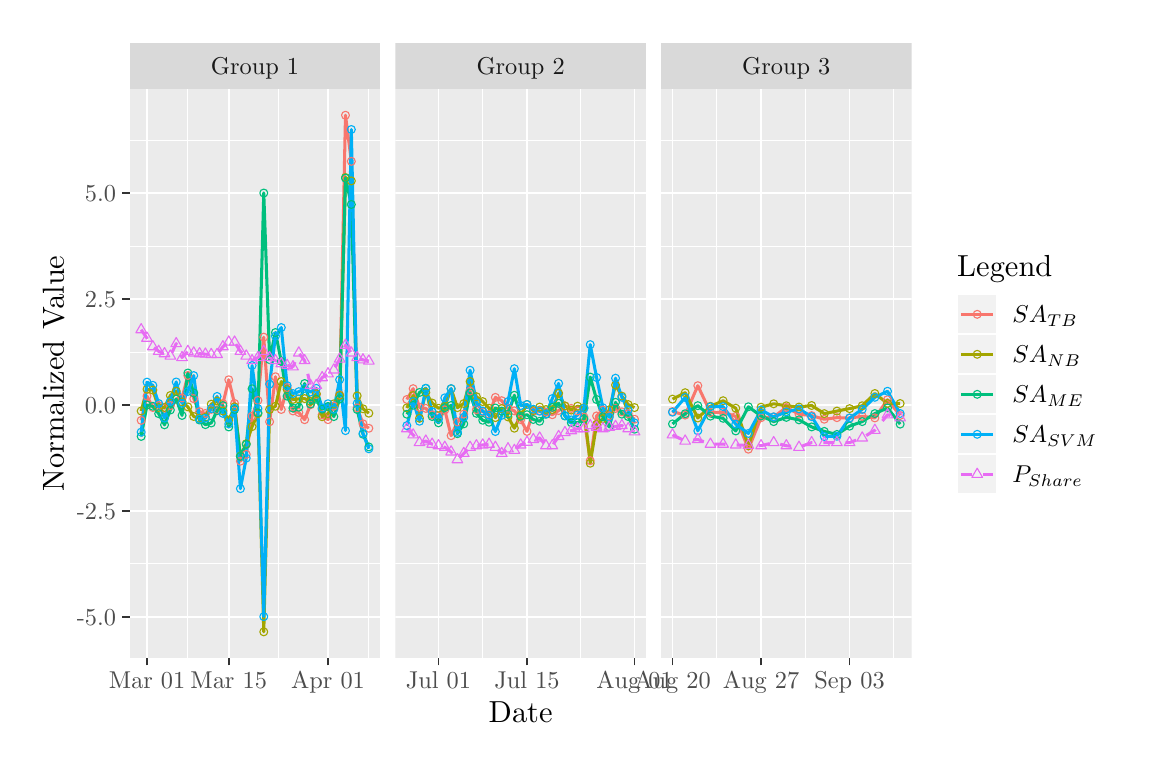
\begin{tikzpicture}[x=1pt,y=1pt]
\definecolor{fillColor}{RGB}{255,255,255}
\path[use as bounding box,fill=fillColor,fill opacity=0.00] (0,0) rectangle (397.48,258.37);
\begin{scope}
\path[clip] (  0.00,  0.00) rectangle (397.48,258.37);
\definecolor{drawColor}{RGB}{255,255,255}
\definecolor{fillColor}{RGB}{255,255,255}

\path[draw=drawColor,line width= 0.6pt,line join=round,line cap=round,fill=fillColor] (  0.00, -0.00) rectangle (397.48,258.37);
\end{scope}
\begin{scope}
\path[clip] ( 36.90, 30.73) rectangle (127.40,236.06);
\definecolor{fillColor}{gray}{0.92}

\path[fill=fillColor] ( 36.90, 30.73) rectangle (127.40,236.06);
\definecolor{drawColor}{RGB}{255,255,255}

\path[draw=drawColor,line width= 0.3pt,line join=round] ( 36.90, 64.64) --
	(127.40, 64.64);

\path[draw=drawColor,line width= 0.3pt,line join=round] ( 36.90,102.91) --
	(127.40,102.91);

\path[draw=drawColor,line width= 0.3pt,line join=round] ( 36.90,141.19) --
	(127.40,141.19);

\path[draw=drawColor,line width= 0.3pt,line join=round] ( 36.90,179.46) --
	(127.40,179.46);

\path[draw=drawColor,line width= 0.3pt,line join=round] ( 36.90,217.73) --
	(127.40,217.73);

\path[draw=drawColor,line width= 0.3pt,line join=round] ( 57.89, 30.73) --
	( 57.89,236.06);

\path[draw=drawColor,line width= 0.3pt,line join=round] ( 90.59, 30.73) --
	( 90.59,236.06);

\path[draw=drawColor,line width= 0.3pt,line join=round] (123.28, 30.73) --
	(123.28,236.06);

\path[draw=drawColor,line width= 0.6pt,line join=round] ( 36.90, 45.50) --
	(127.40, 45.50);

\path[draw=drawColor,line width= 0.6pt,line join=round] ( 36.90, 83.78) --
	(127.40, 83.78);

\path[draw=drawColor,line width= 0.6pt,line join=round] ( 36.90,122.05) --
	(127.40,122.05);

\path[draw=drawColor,line width= 0.6pt,line join=round] ( 36.90,160.32) --
	(127.40,160.32);

\path[draw=drawColor,line width= 0.6pt,line join=round] ( 36.90,198.60) --
	(127.40,198.60);

\path[draw=drawColor,line width= 0.6pt,line join=round] ( 43.12, 30.73) --
	( 43.12,236.06);

\path[draw=drawColor,line width= 0.6pt,line join=round] ( 72.66, 30.73) --
	( 72.66,236.06);

\path[draw=drawColor,line width= 0.6pt,line join=round] (108.52, 30.73) --
	(108.52,236.06);
\definecolor{drawColor}{RGB}{248,118,109}

\path[draw=drawColor,line width= 1.1pt,line join=round] ( 41.01,116.47) --
	( 43.12,125.22) --
	( 45.23,121.11) --
	( 47.34,121.83) --
	( 49.45,120.87) --
	( 51.56,121.81) --
	( 53.67,124.21) --
	( 55.78,124.56) --
	( 57.89,132.69) --
	( 60.00,124.31) --
	( 62.11,119.60) --
	( 64.22,118.95) --
	( 66.33,120.46) --
	( 68.44,120.28) --
	( 70.55,122.55) --
	( 72.66,131.14) --
	( 74.76,122.58) --
	( 76.87,101.72) --
	( 78.98,104.19) --
	( 81.09,117.98) --
	( 83.20,123.68) --
	( 85.31,146.53) --
	( 87.42,115.96) --
	( 89.53,132.24) --
	( 91.64,120.40) --
	( 93.75,128.31) --
	( 95.86,119.87) --
	( 97.97,119.33) --
	(100.08,116.71) --
	(102.19,122.12) --
	(104.30,125.85) --
	(106.41,118.46) --
	(108.52,116.73) --
	(110.63,121.64) --
	(112.73,125.69) --
	(114.84,226.73) --
	(116.95,210.07) --
	(119.06,121.00) --
	(121.17,115.23) --
	(123.28,113.61);
\definecolor{drawColor}{RGB}{163,165,0}

\path[draw=drawColor,line width= 1.1pt,line join=round] ( 41.01,119.85) --
	( 43.12,127.71) --
	( 45.23,127.41) --
	( 47.34,121.13) --
	( 49.45,121.15) --
	( 51.56,125.46) --
	( 53.67,127.03) --
	( 55.78,123.16) --
	( 57.89,121.33) --
	( 60.00,117.87) --
	( 62.11,117.18) --
	( 64.22,117.58) --
	( 66.33,122.31) --
	( 68.44,123.46) --
	( 70.55,119.86) --
	( 72.66,116.56) --
	( 74.76,121.36) --
	( 76.87,103.57) --
	( 78.98,108.02) --
	( 81.09,114.19) --
	( 83.20,118.90) --
	( 85.31, 40.06) --
	( 87.42,120.43) --
	( 89.53,121.56) --
	( 91.64,130.50) --
	( 93.75,127.64) --
	( 95.86,124.03) --
	( 97.97,124.22) --
	(100.08,124.33) --
	(102.19,123.31) --
	(104.30,126.10) --
	(106.41,117.78) --
	(108.52,118.90) --
	(110.63,122.45) --
	(112.73,125.49) --
	(114.84,204.22) --
	(116.95,203.00) --
	(119.06,125.33) --
	(121.17,120.66) --
	(123.28,119.06);
\definecolor{drawColor}{RGB}{0,191,125}

\path[draw=drawColor,line width= 1.1pt,line join=round] ( 41.01,110.67) --
	( 43.12,122.03) --
	( 45.23,121.56) --
	( 47.34,118.89) --
	( 49.45,114.85) --
	( 51.56,120.22) --
	( 53.67,124.17) --
	( 55.78,118.24) --
	( 57.89,133.59) --
	( 60.00,126.40) --
	( 62.11,116.59) --
	( 64.22,114.93) --
	( 66.33,115.52) --
	( 68.44,119.95) --
	( 70.55,121.80) --
	( 72.66,114.09) --
	( 74.76,120.42) --
	( 76.87,103.45) --
	( 78.98,107.79) --
	( 81.09,127.90) --
	( 83.20,119.21) --
	( 85.31,198.62) --
	( 87.42,138.41) --
	( 89.53,148.20) --
	( 91.64,137.77) --
	( 93.75,125.21) --
	( 95.86,120.91) --
	( 97.97,121.24) --
	(100.08,129.78) --
	(102.19,122.37) --
	(104.30,124.09) --
	(106.41,120.53) --
	(108.52,121.50) --
	(110.63,117.83) --
	(112.73,124.20) --
	(114.84,203.99) --
	(116.95,194.49) --
	(119.06,120.38) --
	(121.17,111.47) --
	(123.28,106.87);
\definecolor{drawColor}{RGB}{0,176,246}

\path[draw=drawColor,line width= 1.1pt,line join=round] ( 41.01,112.22) --
	( 43.12,130.28) --
	( 45.23,129.13) --
	( 47.34,122.56) --
	( 49.45,117.31) --
	( 51.56,123.25) --
	( 53.67,130.34) --
	( 55.78,122.64) --
	( 57.89,126.91) --
	( 60.00,132.65) --
	( 62.11,116.92) --
	( 64.22,117.25) --
	( 66.33,120.71) --
	( 68.44,125.11) --
	( 70.55,118.99) --
	( 72.66,115.19) --
	( 74.76,120.86) --
	( 76.87, 91.79) --
	( 78.98,102.83) --
	( 81.09,136.27) --
	( 83.20,120.71) --
	( 85.31, 45.55) --
	( 87.42,129.56) --
	( 89.53,146.92) --
	( 91.64,150.01) --
	( 93.75,129.03) --
	( 95.86,126.15) --
	( 97.97,126.84) --
	(100.08,127.99) --
	(102.19,126.70) --
	(104.30,128.03) --
	(106.41,120.96) --
	(108.52,122.48) --
	(110.63,120.52) --
	(112.73,131.17) --
	(114.84,112.76) --
	(116.95,221.58) --
	(119.06,122.56) --
	(121.17,111.77) --
	(123.28,106.20);
\definecolor{drawColor}{RGB}{231,107,243}

\path[draw=drawColor,line width= 1.1pt,dash pattern=on 4pt off 4pt ,line join=round] ( 41.01,149.23) --
	( 43.12,146.16) --
	( 45.23,143.09) --
	( 47.34,141.41) --
	( 49.45,140.57) --
	( 51.56,139.73) --
	( 53.67,144.20) --
	( 55.78,139.17) --
	( 57.89,141.41) --
	( 60.00,140.85) --
	( 62.11,140.57) --
	( 64.22,140.43) --
	( 66.33,140.29) --
	( 68.44,140.29) --
	( 70.55,143.09) --
	( 72.66,144.76) --
	( 74.76,144.76) --
	( 76.87,141.41) --
	( 78.98,139.73) --
	( 81.09,138.06) --
	( 83.20,139.17) --
	( 85.31,141.41) --
	( 87.42,139.17) --
	( 89.53,138.06) --
	( 91.64,136.94) --
	( 93.75,136.38) --
	( 95.86,135.82) --
	( 97.97,140.85) --
	(100.08,138.06) --
	(102.19,129.11) --
	(104.30,129.11) --
	(106.41,131.91) --
	(108.52,133.30) --
	(110.63,134.70) --
	(112.73,138.61) --
	(114.84,143.64) --
	(116.95,140.85) --
	(119.06,139.17) --
	(121.17,138.33) --
	(123.28,137.92);
\definecolor{drawColor}{RGB}{248,118,109}

\path[draw=drawColor,line width= 0.4pt,line join=round,line cap=round] ( 41.01,116.47) circle (  1.43);

\path[draw=drawColor,line width= 0.4pt,line join=round,line cap=round] ( 43.12,125.22) circle (  1.43);

\path[draw=drawColor,line width= 0.4pt,line join=round,line cap=round] ( 45.23,121.11) circle (  1.43);

\path[draw=drawColor,line width= 0.4pt,line join=round,line cap=round] ( 47.34,121.83) circle (  1.43);

\path[draw=drawColor,line width= 0.4pt,line join=round,line cap=round] ( 49.45,120.87) circle (  1.43);

\path[draw=drawColor,line width= 0.4pt,line join=round,line cap=round] ( 51.56,121.81) circle (  1.43);

\path[draw=drawColor,line width= 0.4pt,line join=round,line cap=round] ( 53.67,124.21) circle (  1.43);

\path[draw=drawColor,line width= 0.4pt,line join=round,line cap=round] ( 55.78,124.56) circle (  1.43);

\path[draw=drawColor,line width= 0.4pt,line join=round,line cap=round] ( 57.89,132.69) circle (  1.43);

\path[draw=drawColor,line width= 0.4pt,line join=round,line cap=round] ( 60.00,124.31) circle (  1.43);

\path[draw=drawColor,line width= 0.4pt,line join=round,line cap=round] ( 62.11,119.60) circle (  1.43);

\path[draw=drawColor,line width= 0.4pt,line join=round,line cap=round] ( 64.22,118.95) circle (  1.43);

\path[draw=drawColor,line width= 0.4pt,line join=round,line cap=round] ( 66.33,120.46) circle (  1.43);

\path[draw=drawColor,line width= 0.4pt,line join=round,line cap=round] ( 68.44,120.28) circle (  1.43);

\path[draw=drawColor,line width= 0.4pt,line join=round,line cap=round] ( 70.55,122.55) circle (  1.43);

\path[draw=drawColor,line width= 0.4pt,line join=round,line cap=round] ( 72.66,131.14) circle (  1.43);

\path[draw=drawColor,line width= 0.4pt,line join=round,line cap=round] ( 74.76,122.58) circle (  1.43);

\path[draw=drawColor,line width= 0.4pt,line join=round,line cap=round] ( 76.87,101.72) circle (  1.43);

\path[draw=drawColor,line width= 0.4pt,line join=round,line cap=round] ( 78.98,104.19) circle (  1.43);

\path[draw=drawColor,line width= 0.4pt,line join=round,line cap=round] ( 81.09,117.98) circle (  1.43);

\path[draw=drawColor,line width= 0.4pt,line join=round,line cap=round] ( 83.20,123.68) circle (  1.43);

\path[draw=drawColor,line width= 0.4pt,line join=round,line cap=round] ( 85.31,146.53) circle (  1.43);

\path[draw=drawColor,line width= 0.4pt,line join=round,line cap=round] ( 87.42,115.96) circle (  1.43);

\path[draw=drawColor,line width= 0.4pt,line join=round,line cap=round] ( 89.53,132.24) circle (  1.43);

\path[draw=drawColor,line width= 0.4pt,line join=round,line cap=round] ( 91.64,120.40) circle (  1.43);

\path[draw=drawColor,line width= 0.4pt,line join=round,line cap=round] ( 93.75,128.31) circle (  1.43);

\path[draw=drawColor,line width= 0.4pt,line join=round,line cap=round] ( 95.86,119.87) circle (  1.43);

\path[draw=drawColor,line width= 0.4pt,line join=round,line cap=round] ( 97.97,119.33) circle (  1.43);

\path[draw=drawColor,line width= 0.4pt,line join=round,line cap=round] (100.08,116.71) circle (  1.43);

\path[draw=drawColor,line width= 0.4pt,line join=round,line cap=round] (102.19,122.12) circle (  1.43);

\path[draw=drawColor,line width= 0.4pt,line join=round,line cap=round] (104.30,125.85) circle (  1.43);

\path[draw=drawColor,line width= 0.4pt,line join=round,line cap=round] (106.41,118.46) circle (  1.43);

\path[draw=drawColor,line width= 0.4pt,line join=round,line cap=round] (108.52,116.73) circle (  1.43);

\path[draw=drawColor,line width= 0.4pt,line join=round,line cap=round] (110.63,121.64) circle (  1.43);

\path[draw=drawColor,line width= 0.4pt,line join=round,line cap=round] (112.73,125.69) circle (  1.43);

\path[draw=drawColor,line width= 0.4pt,line join=round,line cap=round] (114.84,226.73) circle (  1.43);

\path[draw=drawColor,line width= 0.4pt,line join=round,line cap=round] (116.95,210.07) circle (  1.43);

\path[draw=drawColor,line width= 0.4pt,line join=round,line cap=round] (119.06,121.00) circle (  1.43);

\path[draw=drawColor,line width= 0.4pt,line join=round,line cap=round] (121.17,115.23) circle (  1.43);

\path[draw=drawColor,line width= 0.4pt,line join=round,line cap=round] (123.28,113.61) circle (  1.43);
\definecolor{drawColor}{RGB}{163,165,0}

\path[draw=drawColor,line width= 0.4pt,line join=round,line cap=round] ( 41.01,119.85) circle (  1.43);

\path[draw=drawColor,line width= 0.4pt,line join=round,line cap=round] ( 43.12,127.71) circle (  1.43);

\path[draw=drawColor,line width= 0.4pt,line join=round,line cap=round] ( 45.23,127.41) circle (  1.43);

\path[draw=drawColor,line width= 0.4pt,line join=round,line cap=round] ( 47.34,121.13) circle (  1.43);

\path[draw=drawColor,line width= 0.4pt,line join=round,line cap=round] ( 49.45,121.15) circle (  1.43);

\path[draw=drawColor,line width= 0.4pt,line join=round,line cap=round] ( 51.56,125.46) circle (  1.43);

\path[draw=drawColor,line width= 0.4pt,line join=round,line cap=round] ( 53.67,127.03) circle (  1.43);

\path[draw=drawColor,line width= 0.4pt,line join=round,line cap=round] ( 55.78,123.16) circle (  1.43);

\path[draw=drawColor,line width= 0.4pt,line join=round,line cap=round] ( 57.89,121.33) circle (  1.43);

\path[draw=drawColor,line width= 0.4pt,line join=round,line cap=round] ( 60.00,117.87) circle (  1.43);

\path[draw=drawColor,line width= 0.4pt,line join=round,line cap=round] ( 62.11,117.18) circle (  1.43);

\path[draw=drawColor,line width= 0.4pt,line join=round,line cap=round] ( 64.22,117.58) circle (  1.43);

\path[draw=drawColor,line width= 0.4pt,line join=round,line cap=round] ( 66.33,122.31) circle (  1.43);

\path[draw=drawColor,line width= 0.4pt,line join=round,line cap=round] ( 68.44,123.46) circle (  1.43);

\path[draw=drawColor,line width= 0.4pt,line join=round,line cap=round] ( 70.55,119.86) circle (  1.43);

\path[draw=drawColor,line width= 0.4pt,line join=round,line cap=round] ( 72.66,116.56) circle (  1.43);

\path[draw=drawColor,line width= 0.4pt,line join=round,line cap=round] ( 74.76,121.36) circle (  1.43);

\path[draw=drawColor,line width= 0.4pt,line join=round,line cap=round] ( 76.87,103.57) circle (  1.43);

\path[draw=drawColor,line width= 0.4pt,line join=round,line cap=round] ( 78.98,108.02) circle (  1.43);

\path[draw=drawColor,line width= 0.4pt,line join=round,line cap=round] ( 81.09,114.19) circle (  1.43);

\path[draw=drawColor,line width= 0.4pt,line join=round,line cap=round] ( 83.20,118.90) circle (  1.43);

\path[draw=drawColor,line width= 0.4pt,line join=round,line cap=round] ( 85.31, 40.06) circle (  1.43);

\path[draw=drawColor,line width= 0.4pt,line join=round,line cap=round] ( 87.42,120.43) circle (  1.43);

\path[draw=drawColor,line width= 0.4pt,line join=round,line cap=round] ( 89.53,121.56) circle (  1.43);

\path[draw=drawColor,line width= 0.4pt,line join=round,line cap=round] ( 91.64,130.50) circle (  1.43);

\path[draw=drawColor,line width= 0.4pt,line join=round,line cap=round] ( 93.75,127.64) circle (  1.43);

\path[draw=drawColor,line width= 0.4pt,line join=round,line cap=round] ( 95.86,124.03) circle (  1.43);

\path[draw=drawColor,line width= 0.4pt,line join=round,line cap=round] ( 97.97,124.22) circle (  1.43);

\path[draw=drawColor,line width= 0.4pt,line join=round,line cap=round] (100.08,124.33) circle (  1.43);

\path[draw=drawColor,line width= 0.4pt,line join=round,line cap=round] (102.19,123.31) circle (  1.43);

\path[draw=drawColor,line width= 0.4pt,line join=round,line cap=round] (104.30,126.10) circle (  1.43);

\path[draw=drawColor,line width= 0.4pt,line join=round,line cap=round] (106.41,117.78) circle (  1.43);

\path[draw=drawColor,line width= 0.4pt,line join=round,line cap=round] (108.52,118.90) circle (  1.43);

\path[draw=drawColor,line width= 0.4pt,line join=round,line cap=round] (110.63,122.45) circle (  1.43);

\path[draw=drawColor,line width= 0.4pt,line join=round,line cap=round] (112.73,125.49) circle (  1.43);

\path[draw=drawColor,line width= 0.4pt,line join=round,line cap=round] (114.84,204.22) circle (  1.43);

\path[draw=drawColor,line width= 0.4pt,line join=round,line cap=round] (116.95,203.00) circle (  1.43);

\path[draw=drawColor,line width= 0.4pt,line join=round,line cap=round] (119.06,125.33) circle (  1.43);

\path[draw=drawColor,line width= 0.4pt,line join=round,line cap=round] (121.17,120.66) circle (  1.43);

\path[draw=drawColor,line width= 0.4pt,line join=round,line cap=round] (123.28,119.06) circle (  1.43);
\definecolor{drawColor}{RGB}{0,191,125}

\path[draw=drawColor,line width= 0.4pt,line join=round,line cap=round] ( 41.01,110.67) circle (  1.43);

\path[draw=drawColor,line width= 0.4pt,line join=round,line cap=round] ( 43.12,122.03) circle (  1.43);

\path[draw=drawColor,line width= 0.4pt,line join=round,line cap=round] ( 45.23,121.56) circle (  1.43);

\path[draw=drawColor,line width= 0.4pt,line join=round,line cap=round] ( 47.34,118.89) circle (  1.43);

\path[draw=drawColor,line width= 0.4pt,line join=round,line cap=round] ( 49.45,114.85) circle (  1.43);

\path[draw=drawColor,line width= 0.4pt,line join=round,line cap=round] ( 51.56,120.22) circle (  1.43);

\path[draw=drawColor,line width= 0.4pt,line join=round,line cap=round] ( 53.67,124.17) circle (  1.43);

\path[draw=drawColor,line width= 0.4pt,line join=round,line cap=round] ( 55.78,118.24) circle (  1.43);

\path[draw=drawColor,line width= 0.4pt,line join=round,line cap=round] ( 57.89,133.59) circle (  1.43);

\path[draw=drawColor,line width= 0.4pt,line join=round,line cap=round] ( 60.00,126.40) circle (  1.43);

\path[draw=drawColor,line width= 0.4pt,line join=round,line cap=round] ( 62.11,116.59) circle (  1.43);

\path[draw=drawColor,line width= 0.4pt,line join=round,line cap=round] ( 64.22,114.93) circle (  1.43);

\path[draw=drawColor,line width= 0.4pt,line join=round,line cap=round] ( 66.33,115.52) circle (  1.43);

\path[draw=drawColor,line width= 0.4pt,line join=round,line cap=round] ( 68.44,119.95) circle (  1.43);

\path[draw=drawColor,line width= 0.4pt,line join=round,line cap=round] ( 70.55,121.80) circle (  1.43);

\path[draw=drawColor,line width= 0.4pt,line join=round,line cap=round] ( 72.66,114.09) circle (  1.43);

\path[draw=drawColor,line width= 0.4pt,line join=round,line cap=round] ( 74.76,120.42) circle (  1.43);

\path[draw=drawColor,line width= 0.4pt,line join=round,line cap=round] ( 76.87,103.45) circle (  1.43);

\path[draw=drawColor,line width= 0.4pt,line join=round,line cap=round] ( 78.98,107.79) circle (  1.43);

\path[draw=drawColor,line width= 0.4pt,line join=round,line cap=round] ( 81.09,127.90) circle (  1.43);

\path[draw=drawColor,line width= 0.4pt,line join=round,line cap=round] ( 83.20,119.21) circle (  1.43);

\path[draw=drawColor,line width= 0.4pt,line join=round,line cap=round] ( 85.31,198.62) circle (  1.43);

\path[draw=drawColor,line width= 0.4pt,line join=round,line cap=round] ( 87.42,138.41) circle (  1.43);

\path[draw=drawColor,line width= 0.4pt,line join=round,line cap=round] ( 89.53,148.20) circle (  1.43);

\path[draw=drawColor,line width= 0.4pt,line join=round,line cap=round] ( 91.64,137.77) circle (  1.43);

\path[draw=drawColor,line width= 0.4pt,line join=round,line cap=round] ( 93.75,125.21) circle (  1.43);

\path[draw=drawColor,line width= 0.4pt,line join=round,line cap=round] ( 95.86,120.91) circle (  1.43);

\path[draw=drawColor,line width= 0.4pt,line join=round,line cap=round] ( 97.97,121.24) circle (  1.43);

\path[draw=drawColor,line width= 0.4pt,line join=round,line cap=round] (100.08,129.78) circle (  1.43);

\path[draw=drawColor,line width= 0.4pt,line join=round,line cap=round] (102.19,122.37) circle (  1.43);

\path[draw=drawColor,line width= 0.4pt,line join=round,line cap=round] (104.30,124.09) circle (  1.43);

\path[draw=drawColor,line width= 0.4pt,line join=round,line cap=round] (106.41,120.53) circle (  1.43);

\path[draw=drawColor,line width= 0.4pt,line join=round,line cap=round] (108.52,121.50) circle (  1.43);

\path[draw=drawColor,line width= 0.4pt,line join=round,line cap=round] (110.63,117.83) circle (  1.43);

\path[draw=drawColor,line width= 0.4pt,line join=round,line cap=round] (112.73,124.20) circle (  1.43);

\path[draw=drawColor,line width= 0.4pt,line join=round,line cap=round] (114.84,203.99) circle (  1.43);

\path[draw=drawColor,line width= 0.4pt,line join=round,line cap=round] (116.95,194.49) circle (  1.43);

\path[draw=drawColor,line width= 0.4pt,line join=round,line cap=round] (119.06,120.38) circle (  1.43);

\path[draw=drawColor,line width= 0.4pt,line join=round,line cap=round] (121.17,111.47) circle (  1.43);

\path[draw=drawColor,line width= 0.4pt,line join=round,line cap=round] (123.28,106.87) circle (  1.43);
\definecolor{drawColor}{RGB}{0,176,246}

\path[draw=drawColor,line width= 0.4pt,line join=round,line cap=round] ( 41.01,112.22) circle (  1.43);

\path[draw=drawColor,line width= 0.4pt,line join=round,line cap=round] ( 43.12,130.28) circle (  1.43);

\path[draw=drawColor,line width= 0.4pt,line join=round,line cap=round] ( 45.23,129.13) circle (  1.43);

\path[draw=drawColor,line width= 0.4pt,line join=round,line cap=round] ( 47.34,122.56) circle (  1.43);

\path[draw=drawColor,line width= 0.4pt,line join=round,line cap=round] ( 49.45,117.31) circle (  1.43);

\path[draw=drawColor,line width= 0.4pt,line join=round,line cap=round] ( 51.56,123.25) circle (  1.43);

\path[draw=drawColor,line width= 0.4pt,line join=round,line cap=round] ( 53.67,130.34) circle (  1.43);

\path[draw=drawColor,line width= 0.4pt,line join=round,line cap=round] ( 55.78,122.64) circle (  1.43);

\path[draw=drawColor,line width= 0.4pt,line join=round,line cap=round] ( 57.89,126.91) circle (  1.43);

\path[draw=drawColor,line width= 0.4pt,line join=round,line cap=round] ( 60.00,132.65) circle (  1.43);

\path[draw=drawColor,line width= 0.4pt,line join=round,line cap=round] ( 62.11,116.92) circle (  1.43);

\path[draw=drawColor,line width= 0.4pt,line join=round,line cap=round] ( 64.22,117.25) circle (  1.43);

\path[draw=drawColor,line width= 0.4pt,line join=round,line cap=round] ( 66.33,120.71) circle (  1.43);

\path[draw=drawColor,line width= 0.4pt,line join=round,line cap=round] ( 68.44,125.11) circle (  1.43);

\path[draw=drawColor,line width= 0.4pt,line join=round,line cap=round] ( 70.55,118.99) circle (  1.43);

\path[draw=drawColor,line width= 0.4pt,line join=round,line cap=round] ( 72.66,115.19) circle (  1.43);

\path[draw=drawColor,line width= 0.4pt,line join=round,line cap=round] ( 74.76,120.86) circle (  1.43);

\path[draw=drawColor,line width= 0.4pt,line join=round,line cap=round] ( 76.87, 91.79) circle (  1.43);

\path[draw=drawColor,line width= 0.4pt,line join=round,line cap=round] ( 78.98,102.83) circle (  1.43);

\path[draw=drawColor,line width= 0.4pt,line join=round,line cap=round] ( 81.09,136.27) circle (  1.43);

\path[draw=drawColor,line width= 0.4pt,line join=round,line cap=round] ( 83.20,120.71) circle (  1.43);

\path[draw=drawColor,line width= 0.4pt,line join=round,line cap=round] ( 85.31, 45.55) circle (  1.43);

\path[draw=drawColor,line width= 0.4pt,line join=round,line cap=round] ( 87.42,129.56) circle (  1.43);

\path[draw=drawColor,line width= 0.4pt,line join=round,line cap=round] ( 89.53,146.92) circle (  1.43);

\path[draw=drawColor,line width= 0.4pt,line join=round,line cap=round] ( 91.64,150.01) circle (  1.43);

\path[draw=drawColor,line width= 0.4pt,line join=round,line cap=round] ( 93.75,129.03) circle (  1.43);

\path[draw=drawColor,line width= 0.4pt,line join=round,line cap=round] ( 95.86,126.15) circle (  1.43);

\path[draw=drawColor,line width= 0.4pt,line join=round,line cap=round] ( 97.97,126.84) circle (  1.43);

\path[draw=drawColor,line width= 0.4pt,line join=round,line cap=round] (100.08,127.99) circle (  1.43);

\path[draw=drawColor,line width= 0.4pt,line join=round,line cap=round] (102.19,126.70) circle (  1.43);

\path[draw=drawColor,line width= 0.4pt,line join=round,line cap=round] (104.30,128.03) circle (  1.43);

\path[draw=drawColor,line width= 0.4pt,line join=round,line cap=round] (106.41,120.96) circle (  1.43);

\path[draw=drawColor,line width= 0.4pt,line join=round,line cap=round] (108.52,122.48) circle (  1.43);

\path[draw=drawColor,line width= 0.4pt,line join=round,line cap=round] (110.63,120.52) circle (  1.43);

\path[draw=drawColor,line width= 0.4pt,line join=round,line cap=round] (112.73,131.17) circle (  1.43);

\path[draw=drawColor,line width= 0.4pt,line join=round,line cap=round] (114.84,112.76) circle (  1.43);

\path[draw=drawColor,line width= 0.4pt,line join=round,line cap=round] (116.95,221.58) circle (  1.43);

\path[draw=drawColor,line width= 0.4pt,line join=round,line cap=round] (119.06,122.56) circle (  1.43);

\path[draw=drawColor,line width= 0.4pt,line join=round,line cap=round] (121.17,111.77) circle (  1.43);

\path[draw=drawColor,line width= 0.4pt,line join=round,line cap=round] (123.28,106.20) circle (  1.43);
\definecolor{drawColor}{RGB}{231,107,243}

\path[draw=drawColor,line width= 0.4pt,line join=round,line cap=round] ( 41.01,151.45) --
	( 42.93,148.13) --
	( 39.09,148.13) --
	( 41.01,151.45);

\path[draw=drawColor,line width= 0.4pt,line join=round,line cap=round] ( 43.12,148.38) --
	( 45.04,145.05) --
	( 41.20,145.05) --
	( 43.12,148.38);

\path[draw=drawColor,line width= 0.4pt,line join=round,line cap=round] ( 45.23,145.30) --
	( 47.15,141.98) --
	( 43.31,141.98) --
	( 45.23,145.30);

\path[draw=drawColor,line width= 0.4pt,line join=round,line cap=round] ( 47.34,143.63) --
	( 49.26,140.30) --
	( 45.42,140.30) --
	( 47.34,143.63);

\path[draw=drawColor,line width= 0.4pt,line join=round,line cap=round] ( 49.45,142.79) --
	( 51.37,139.46) --
	( 47.53,139.46) --
	( 49.45,142.79);

\path[draw=drawColor,line width= 0.4pt,line join=round,line cap=round] ( 51.56,141.95) --
	( 53.48,138.62) --
	( 49.64,138.62) --
	( 51.56,141.95);

\path[draw=drawColor,line width= 0.4pt,line join=round,line cap=round] ( 53.67,146.42) --
	( 55.59,143.09) --
	( 51.75,143.09) --
	( 53.67,146.42);

\path[draw=drawColor,line width= 0.4pt,line join=round,line cap=round] ( 55.78,141.39) --
	( 57.70,138.06) --
	( 53.86,138.06) --
	( 55.78,141.39);

\path[draw=drawColor,line width= 0.4pt,line join=round,line cap=round] ( 57.89,143.63) --
	( 59.81,140.30) --
	( 55.97,140.30) --
	( 57.89,143.63);

\path[draw=drawColor,line width= 0.4pt,line join=round,line cap=round] ( 60.00,143.07) --
	( 61.92,139.74) --
	( 58.08,139.74) --
	( 60.00,143.07);

\path[draw=drawColor,line width= 0.4pt,line join=round,line cap=round] ( 62.11,142.79) --
	( 64.03,139.46) --
	( 60.19,139.46) --
	( 62.11,142.79);

\path[draw=drawColor,line width= 0.4pt,line join=round,line cap=round] ( 64.22,142.65) --
	( 66.14,139.32) --
	( 62.30,139.32) --
	( 64.22,142.65);

\path[draw=drawColor,line width= 0.4pt,line join=round,line cap=round] ( 66.33,142.51) --
	( 68.25,139.18) --
	( 64.41,139.18) --
	( 66.33,142.51);

\path[draw=drawColor,line width= 0.4pt,line join=round,line cap=round] ( 68.44,142.51) --
	( 70.36,139.18) --
	( 66.51,139.18) --
	( 68.44,142.51);

\path[draw=drawColor,line width= 0.4pt,line join=round,line cap=round] ( 70.55,145.30) --
	( 72.47,141.98) --
	( 68.62,141.98) --
	( 70.55,145.30);

\path[draw=drawColor,line width= 0.4pt,line join=round,line cap=round] ( 72.66,146.98) --
	( 74.58,143.65) --
	( 70.73,143.65) --
	( 72.66,146.98);

\path[draw=drawColor,line width= 0.4pt,line join=round,line cap=round] ( 74.76,146.98) --
	( 76.69,143.65) --
	( 72.84,143.65) --
	( 74.76,146.98);

\path[draw=drawColor,line width= 0.4pt,line join=round,line cap=round] ( 76.87,143.63) --
	( 78.80,140.30) --
	( 74.95,140.30) --
	( 76.87,143.63);

\path[draw=drawColor,line width= 0.4pt,line join=round,line cap=round] ( 78.98,141.95) --
	( 80.90,138.62) --
	( 77.06,138.62) --
	( 78.98,141.95);

\path[draw=drawColor,line width= 0.4pt,line join=round,line cap=round] ( 81.09,140.27) --
	( 83.01,136.95) --
	( 79.17,136.95) --
	( 81.09,140.27);

\path[draw=drawColor,line width= 0.4pt,line join=round,line cap=round] ( 83.20,141.39) --
	( 85.12,138.06) --
	( 81.28,138.06) --
	( 83.20,141.39);

\path[draw=drawColor,line width= 0.4pt,line join=round,line cap=round] ( 85.31,143.63) --
	( 87.23,140.30) --
	( 83.39,140.30) --
	( 85.31,143.63);

\path[draw=drawColor,line width= 0.4pt,line join=round,line cap=round] ( 87.42,141.39) --
	( 89.34,138.06) --
	( 85.50,138.06) --
	( 87.42,141.39);

\path[draw=drawColor,line width= 0.4pt,line join=round,line cap=round] ( 89.53,140.27) --
	( 91.45,136.95) --
	( 87.61,136.95) --
	( 89.53,140.27);

\path[draw=drawColor,line width= 0.4pt,line join=round,line cap=round] ( 91.64,139.16) --
	( 93.56,135.83) --
	( 89.72,135.83) --
	( 91.64,139.16);

\path[draw=drawColor,line width= 0.4pt,line join=round,line cap=round] ( 93.75,138.60) --
	( 95.67,135.27) --
	( 91.83,135.27) --
	( 93.75,138.60);

\path[draw=drawColor,line width= 0.4pt,line join=round,line cap=round] ( 95.86,138.04) --
	( 97.78,134.71) --
	( 93.94,134.71) --
	( 95.86,138.04);

\path[draw=drawColor,line width= 0.4pt,line join=round,line cap=round] ( 97.97,143.07) --
	( 99.89,139.74) --
	( 96.05,139.74) --
	( 97.97,143.07);

\path[draw=drawColor,line width= 0.4pt,line join=round,line cap=round] (100.08,140.27) --
	(102.00,136.95) --
	( 98.16,136.95) --
	(100.08,140.27);

\path[draw=drawColor,line width= 0.4pt,line join=round,line cap=round] (102.19,131.33) --
	(104.11,128.00) --
	(100.27,128.00) --
	(102.19,131.33);

\path[draw=drawColor,line width= 0.4pt,line join=round,line cap=round] (104.30,131.33) --
	(106.22,128.00) --
	(102.38,128.00) --
	(104.30,131.33);

\path[draw=drawColor,line width= 0.4pt,line join=round,line cap=round] (106.41,134.12) --
	(108.33,130.80) --
	(104.49,130.80) --
	(106.41,134.12);

\path[draw=drawColor,line width= 0.4pt,line join=round,line cap=round] (108.52,135.52) --
	(110.44,132.19) --
	(106.59,132.19) --
	(108.52,135.52);

\path[draw=drawColor,line width= 0.4pt,line join=round,line cap=round] (110.63,136.92) --
	(112.55,133.59) --
	(108.70,133.59) --
	(110.63,136.92);

\path[draw=drawColor,line width= 0.4pt,line join=round,line cap=round] (112.73,140.83) --
	(114.66,137.50) --
	(110.81,137.50) --
	(112.73,140.83);

\path[draw=drawColor,line width= 0.4pt,line join=round,line cap=round] (114.84,145.86) --
	(116.77,142.54) --
	(112.92,142.54) --
	(114.84,145.86);

\path[draw=drawColor,line width= 0.4pt,line join=round,line cap=round] (116.95,143.07) --
	(118.88,139.74) --
	(115.03,139.74) --
	(116.95,143.07);

\path[draw=drawColor,line width= 0.4pt,line join=round,line cap=round] (119.06,141.39) --
	(120.98,138.06) --
	(117.14,138.06) --
	(119.06,141.39);

\path[draw=drawColor,line width= 0.4pt,line join=round,line cap=round] (121.17,140.55) --
	(123.09,137.23) --
	(119.25,137.23) --
	(121.17,140.55);

\path[draw=drawColor,line width= 0.4pt,line join=round,line cap=round] (123.28,140.13) --
	(125.20,136.81) --
	(121.36,136.81) --
	(123.28,140.13);
\end{scope}
\begin{scope}
\path[clip] (132.90, 30.73) rectangle (223.39,236.06);
\definecolor{fillColor}{gray}{0.92}

\path[fill=fillColor] (132.90, 30.73) rectangle (223.39,236.06);
\definecolor{drawColor}{RGB}{255,255,255}

\path[draw=drawColor,line width= 0.3pt,line join=round] (132.90, 64.64) --
	(223.39, 64.64);

\path[draw=drawColor,line width= 0.3pt,line join=round] (132.90,102.91) --
	(223.39,102.91);

\path[draw=drawColor,line width= 0.3pt,line join=round] (132.90,141.19) --
	(223.39,141.19);

\path[draw=drawColor,line width= 0.3pt,line join=round] (132.90,179.46) --
	(223.39,179.46);

\path[draw=drawColor,line width= 0.3pt,line join=round] (132.90,217.73) --
	(223.39,217.73);

\path[draw=drawColor,line width= 0.3pt,line join=round] (164.43, 30.73) --
	(164.43,236.06);

\path[draw=drawColor,line width= 0.3pt,line join=round] (199.85, 30.73) --
	(199.85,236.06);

\path[draw=drawColor,line width= 0.6pt,line join=round] (132.90, 45.50) --
	(223.39, 45.50);

\path[draw=drawColor,line width= 0.6pt,line join=round] (132.90, 83.78) --
	(223.39, 83.78);

\path[draw=drawColor,line width= 0.6pt,line join=round] (132.90,122.05) --
	(223.39,122.05);

\path[draw=drawColor,line width= 0.6pt,line join=round] (132.90,160.32) --
	(223.39,160.32);

\path[draw=drawColor,line width= 0.6pt,line join=round] (132.90,198.60) --
	(223.39,198.60);

\path[draw=drawColor,line width= 0.6pt,line join=round] (148.44, 30.73) --
	(148.44,236.06);

\path[draw=drawColor,line width= 0.6pt,line join=round] (180.43, 30.73) --
	(180.43,236.06);

\path[draw=drawColor,line width= 0.6pt,line join=round] (219.28, 30.73) --
	(219.28,236.06);
\definecolor{drawColor}{RGB}{248,118,109}

\path[draw=drawColor,line width= 1.1pt,line join=round] (137.01,124.01) --
	(139.29,127.93) --
	(141.58,121.19) --
	(143.86,120.79) --
	(146.15,118.44) --
	(148.44,118.07) --
	(150.72,120.24) --
	(153.01,110.94) --
	(155.29,115.89) --
	(157.58,118.74) --
	(159.86,127.07) --
	(162.15,120.34) --
	(164.43,119.55) --
	(166.72,118.65) --
	(169.00,124.78) --
	(171.29,123.58) --
	(173.57,120.78) --
	(175.86,119.91) --
	(178.14,116.76) --
	(180.43,112.49) --
	(182.71,119.70) --
	(185.00,119.94) --
	(187.28,119.41) --
	(189.57,118.51) --
	(191.86,120.02) --
	(194.14,121.66) --
	(196.43,120.79) --
	(198.71,119.87) --
	(201.00,117.65) --
	(203.28,101.90) --
	(205.57,118.07) --
	(207.85,120.22) --
	(210.14,118.11) --
	(212.42,120.79) --
	(214.71,119.56) --
	(216.99,118.88) --
	(219.28,116.88);
\definecolor{drawColor}{RGB}{163,165,0}

\path[draw=drawColor,line width= 1.1pt,line join=round] (137.01,120.96) --
	(139.29,125.47) --
	(141.58,117.22) --
	(143.86,126.57) --
	(146.15,122.74) --
	(148.44,120.85) --
	(150.72,121.54) --
	(153.01,127.89) --
	(155.29,121.07) --
	(157.58,122.54) --
	(159.86,130.50) --
	(162.15,125.03) --
	(164.43,123.25) --
	(166.72,120.85) --
	(169.00,117.47) --
	(171.29,120.72) --
	(173.57,117.71) --
	(175.86,113.63) --
	(178.14,118.32) --
	(180.43,122.21) --
	(182.71,120.05) --
	(185.00,121.27) --
	(187.28,120.38) --
	(189.57,120.36) --
	(191.86,126.29) --
	(194.14,121.69) --
	(196.43,120.19) --
	(198.71,121.60) --
	(201.00,121.00) --
	(203.28,100.98) --
	(205.57,115.00) --
	(207.85,117.07) --
	(210.14,120.26) --
	(212.42,129.24) --
	(214.71,125.22) --
	(216.99,122.18) --
	(219.28,121.09);
\definecolor{drawColor}{RGB}{0,191,125}

\path[draw=drawColor,line width= 1.1pt,line join=round] (137.01,118.69) --
	(139.29,121.92) --
	(141.58,126.55) --
	(143.86,128.03) --
	(146.15,117.86) --
	(148.44,115.58) --
	(150.72,121.06) --
	(153.01,121.83) --
	(155.29,111.65) --
	(157.58,115.20) --
	(159.86,126.38) --
	(162.15,119.02) --
	(164.43,116.50) --
	(166.72,115.78) --
	(169.00,120.94) --
	(171.29,119.80) --
	(173.57,118.74) --
	(175.86,125.54) --
	(178.14,117.96) --
	(180.43,118.51) --
	(182.71,116.79) --
	(185.00,116.14) --
	(187.28,118.68) --
	(189.57,121.17) --
	(191.86,122.64) --
	(194.14,118.04) --
	(196.43,115.61) --
	(198.71,115.60) --
	(201.00,116.94) --
	(203.28,132.13) --
	(205.57,124.01) --
	(207.85,117.75) --
	(210.14,114.09) --
	(212.42,122.99) --
	(214.71,118.71) --
	(216.99,117.84) --
	(219.28,113.27);
\definecolor{drawColor}{RGB}{0,176,246}

\path[draw=drawColor,line width= 1.1pt,line join=round] (137.01,114.57) --
	(139.29,123.29) --
	(141.58,116.15) --
	(143.86,128.07) --
	(146.15,119.63) --
	(148.44,116.94) --
	(150.72,124.60) --
	(153.01,127.94) --
	(155.29,112.16) --
	(157.58,117.59) --
	(159.86,134.58) --
	(162.15,122.94) --
	(164.43,119.83) --
	(166.72,118.33) --
	(169.00,112.43) --
	(171.29,118.28) --
	(173.57,123.26) --
	(175.86,135.14) --
	(178.14,121.80) --
	(180.43,122.19) --
	(182.71,120.51) --
	(185.00,119.77) --
	(187.28,118.78) --
	(189.57,124.33) --
	(191.86,129.83) --
	(194.14,118.19) --
	(196.43,116.64) --
	(198.71,118.43) --
	(201.00,120.84) --
	(203.28,143.84) --
	(205.57,131.96) --
	(207.85,121.02) --
	(210.14,117.60) --
	(212.42,131.71) --
	(214.71,124.81) --
	(216.99,120.20) --
	(219.28,115.56);
\definecolor{drawColor}{RGB}{231,107,243}

\path[draw=drawColor,line width= 1.1pt,dash pattern=on 4pt off 4pt ,line join=round] (137.01,113.46) --
	(139.29,111.22) --
	(141.58,108.43) --
	(143.86,108.99) --
	(146.15,107.87) --
	(148.44,107.31) --
	(150.72,106.75) --
	(153.01,105.08) --
	(155.29,102.28) --
	(157.58,104.52) --
	(159.86,106.75) --
	(162.15,107.31) --
	(164.43,107.59) --
	(166.72,107.87) --
	(169.00,106.75) --
	(171.29,104.52) --
	(173.57,106.19) --
	(175.86,105.63) --
	(178.14,107.59) --
	(180.43,108.57) --
	(182.71,109.55) --
	(185.00,110.11) --
	(187.28,107.31) --
	(189.57,107.31) --
	(191.86,110.67) --
	(194.14,112.06) --
	(196.43,112.76) --
	(198.71,113.46) --
	(201.00,113.46) --
	(203.28,114.58) --
	(205.57,114.02) --
	(207.85,113.46) --
	(210.14,114.02) --
	(212.42,114.30) --
	(214.71,114.58) --
	(216.99,113.46) --
	(219.28,112.34);
\definecolor{drawColor}{RGB}{248,118,109}

\path[draw=drawColor,line width= 0.4pt,line join=round,line cap=round] (137.01,124.01) circle (  1.43);

\path[draw=drawColor,line width= 0.4pt,line join=round,line cap=round] (139.29,127.93) circle (  1.43);

\path[draw=drawColor,line width= 0.4pt,line join=round,line cap=round] (141.58,121.19) circle (  1.43);

\path[draw=drawColor,line width= 0.4pt,line join=round,line cap=round] (143.86,120.79) circle (  1.43);

\path[draw=drawColor,line width= 0.4pt,line join=round,line cap=round] (146.15,118.44) circle (  1.43);

\path[draw=drawColor,line width= 0.4pt,line join=round,line cap=round] (148.44,118.07) circle (  1.43);

\path[draw=drawColor,line width= 0.4pt,line join=round,line cap=round] (150.72,120.24) circle (  1.43);

\path[draw=drawColor,line width= 0.4pt,line join=round,line cap=round] (153.01,110.94) circle (  1.43);

\path[draw=drawColor,line width= 0.4pt,line join=round,line cap=round] (155.29,115.89) circle (  1.43);

\path[draw=drawColor,line width= 0.4pt,line join=round,line cap=round] (157.58,118.74) circle (  1.43);

\path[draw=drawColor,line width= 0.4pt,line join=round,line cap=round] (159.86,127.07) circle (  1.43);

\path[draw=drawColor,line width= 0.4pt,line join=round,line cap=round] (162.15,120.34) circle (  1.43);

\path[draw=drawColor,line width= 0.4pt,line join=round,line cap=round] (164.43,119.55) circle (  1.43);

\path[draw=drawColor,line width= 0.4pt,line join=round,line cap=round] (166.72,118.65) circle (  1.43);

\path[draw=drawColor,line width= 0.4pt,line join=round,line cap=round] (169.00,124.78) circle (  1.43);

\path[draw=drawColor,line width= 0.4pt,line join=round,line cap=round] (171.29,123.58) circle (  1.43);

\path[draw=drawColor,line width= 0.4pt,line join=round,line cap=round] (173.57,120.78) circle (  1.43);

\path[draw=drawColor,line width= 0.4pt,line join=round,line cap=round] (175.86,119.91) circle (  1.43);

\path[draw=drawColor,line width= 0.4pt,line join=round,line cap=round] (178.14,116.76) circle (  1.43);

\path[draw=drawColor,line width= 0.4pt,line join=round,line cap=round] (180.43,112.49) circle (  1.43);

\path[draw=drawColor,line width= 0.4pt,line join=round,line cap=round] (182.71,119.70) circle (  1.43);

\path[draw=drawColor,line width= 0.4pt,line join=round,line cap=round] (185.00,119.94) circle (  1.43);

\path[draw=drawColor,line width= 0.4pt,line join=round,line cap=round] (187.28,119.41) circle (  1.43);

\path[draw=drawColor,line width= 0.4pt,line join=round,line cap=round] (189.57,118.51) circle (  1.43);

\path[draw=drawColor,line width= 0.4pt,line join=round,line cap=round] (191.86,120.02) circle (  1.43);

\path[draw=drawColor,line width= 0.4pt,line join=round,line cap=round] (194.14,121.66) circle (  1.43);

\path[draw=drawColor,line width= 0.4pt,line join=round,line cap=round] (196.43,120.79) circle (  1.43);

\path[draw=drawColor,line width= 0.4pt,line join=round,line cap=round] (198.71,119.87) circle (  1.43);

\path[draw=drawColor,line width= 0.4pt,line join=round,line cap=round] (201.00,117.65) circle (  1.43);

\path[draw=drawColor,line width= 0.4pt,line join=round,line cap=round] (203.28,101.90) circle (  1.43);

\path[draw=drawColor,line width= 0.4pt,line join=round,line cap=round] (205.57,118.07) circle (  1.43);

\path[draw=drawColor,line width= 0.4pt,line join=round,line cap=round] (207.85,120.22) circle (  1.43);

\path[draw=drawColor,line width= 0.4pt,line join=round,line cap=round] (210.14,118.11) circle (  1.43);

\path[draw=drawColor,line width= 0.4pt,line join=round,line cap=round] (212.42,120.79) circle (  1.43);

\path[draw=drawColor,line width= 0.4pt,line join=round,line cap=round] (214.71,119.56) circle (  1.43);

\path[draw=drawColor,line width= 0.4pt,line join=round,line cap=round] (216.99,118.88) circle (  1.43);

\path[draw=drawColor,line width= 0.4pt,line join=round,line cap=round] (219.28,116.88) circle (  1.43);
\definecolor{drawColor}{RGB}{163,165,0}

\path[draw=drawColor,line width= 0.4pt,line join=round,line cap=round] (137.01,120.96) circle (  1.43);

\path[draw=drawColor,line width= 0.4pt,line join=round,line cap=round] (139.29,125.47) circle (  1.43);

\path[draw=drawColor,line width= 0.4pt,line join=round,line cap=round] (141.58,117.22) circle (  1.43);

\path[draw=drawColor,line width= 0.4pt,line join=round,line cap=round] (143.86,126.57) circle (  1.43);

\path[draw=drawColor,line width= 0.4pt,line join=round,line cap=round] (146.15,122.74) circle (  1.43);

\path[draw=drawColor,line width= 0.4pt,line join=round,line cap=round] (148.44,120.85) circle (  1.43);

\path[draw=drawColor,line width= 0.4pt,line join=round,line cap=round] (150.72,121.54) circle (  1.43);

\path[draw=drawColor,line width= 0.4pt,line join=round,line cap=round] (153.01,127.89) circle (  1.43);

\path[draw=drawColor,line width= 0.4pt,line join=round,line cap=round] (155.29,121.07) circle (  1.43);

\path[draw=drawColor,line width= 0.4pt,line join=round,line cap=round] (157.58,122.54) circle (  1.43);

\path[draw=drawColor,line width= 0.4pt,line join=round,line cap=round] (159.86,130.50) circle (  1.43);

\path[draw=drawColor,line width= 0.4pt,line join=round,line cap=round] (162.15,125.03) circle (  1.43);

\path[draw=drawColor,line width= 0.4pt,line join=round,line cap=round] (164.43,123.25) circle (  1.43);

\path[draw=drawColor,line width= 0.4pt,line join=round,line cap=round] (166.72,120.85) circle (  1.43);

\path[draw=drawColor,line width= 0.4pt,line join=round,line cap=round] (169.00,117.47) circle (  1.43);

\path[draw=drawColor,line width= 0.4pt,line join=round,line cap=round] (171.29,120.72) circle (  1.43);

\path[draw=drawColor,line width= 0.4pt,line join=round,line cap=round] (173.57,117.71) circle (  1.43);

\path[draw=drawColor,line width= 0.4pt,line join=round,line cap=round] (175.86,113.63) circle (  1.43);

\path[draw=drawColor,line width= 0.4pt,line join=round,line cap=round] (178.14,118.32) circle (  1.43);

\path[draw=drawColor,line width= 0.4pt,line join=round,line cap=round] (180.43,122.21) circle (  1.43);

\path[draw=drawColor,line width= 0.4pt,line join=round,line cap=round] (182.71,120.05) circle (  1.43);

\path[draw=drawColor,line width= 0.4pt,line join=round,line cap=round] (185.00,121.27) circle (  1.43);

\path[draw=drawColor,line width= 0.4pt,line join=round,line cap=round] (187.28,120.38) circle (  1.43);

\path[draw=drawColor,line width= 0.4pt,line join=round,line cap=round] (189.57,120.36) circle (  1.43);

\path[draw=drawColor,line width= 0.4pt,line join=round,line cap=round] (191.86,126.29) circle (  1.43);

\path[draw=drawColor,line width= 0.4pt,line join=round,line cap=round] (194.14,121.69) circle (  1.43);

\path[draw=drawColor,line width= 0.4pt,line join=round,line cap=round] (196.43,120.19) circle (  1.43);

\path[draw=drawColor,line width= 0.4pt,line join=round,line cap=round] (198.71,121.60) circle (  1.43);

\path[draw=drawColor,line width= 0.4pt,line join=round,line cap=round] (201.00,121.00) circle (  1.43);

\path[draw=drawColor,line width= 0.4pt,line join=round,line cap=round] (203.28,100.98) circle (  1.43);

\path[draw=drawColor,line width= 0.4pt,line join=round,line cap=round] (205.57,115.00) circle (  1.43);

\path[draw=drawColor,line width= 0.4pt,line join=round,line cap=round] (207.85,117.07) circle (  1.43);

\path[draw=drawColor,line width= 0.4pt,line join=round,line cap=round] (210.14,120.26) circle (  1.43);

\path[draw=drawColor,line width= 0.4pt,line join=round,line cap=round] (212.42,129.24) circle (  1.43);

\path[draw=drawColor,line width= 0.4pt,line join=round,line cap=round] (214.71,125.22) circle (  1.43);

\path[draw=drawColor,line width= 0.4pt,line join=round,line cap=round] (216.99,122.18) circle (  1.43);

\path[draw=drawColor,line width= 0.4pt,line join=round,line cap=round] (219.28,121.09) circle (  1.43);
\definecolor{drawColor}{RGB}{0,191,125}

\path[draw=drawColor,line width= 0.4pt,line join=round,line cap=round] (137.01,118.69) circle (  1.43);

\path[draw=drawColor,line width= 0.4pt,line join=round,line cap=round] (139.29,121.92) circle (  1.43);

\path[draw=drawColor,line width= 0.4pt,line join=round,line cap=round] (141.58,126.55) circle (  1.43);

\path[draw=drawColor,line width= 0.4pt,line join=round,line cap=round] (143.86,128.03) circle (  1.43);

\path[draw=drawColor,line width= 0.4pt,line join=round,line cap=round] (146.15,117.86) circle (  1.43);

\path[draw=drawColor,line width= 0.4pt,line join=round,line cap=round] (148.44,115.58) circle (  1.43);

\path[draw=drawColor,line width= 0.4pt,line join=round,line cap=round] (150.72,121.06) circle (  1.43);

\path[draw=drawColor,line width= 0.4pt,line join=round,line cap=round] (153.01,121.83) circle (  1.43);

\path[draw=drawColor,line width= 0.4pt,line join=round,line cap=round] (155.29,111.65) circle (  1.43);

\path[draw=drawColor,line width= 0.4pt,line join=round,line cap=round] (157.58,115.20) circle (  1.43);

\path[draw=drawColor,line width= 0.4pt,line join=round,line cap=round] (159.86,126.38) circle (  1.43);

\path[draw=drawColor,line width= 0.4pt,line join=round,line cap=round] (162.15,119.02) circle (  1.43);

\path[draw=drawColor,line width= 0.4pt,line join=round,line cap=round] (164.43,116.50) circle (  1.43);

\path[draw=drawColor,line width= 0.4pt,line join=round,line cap=round] (166.72,115.78) circle (  1.43);

\path[draw=drawColor,line width= 0.4pt,line join=round,line cap=round] (169.00,120.94) circle (  1.43);

\path[draw=drawColor,line width= 0.4pt,line join=round,line cap=round] (171.29,119.80) circle (  1.43);

\path[draw=drawColor,line width= 0.4pt,line join=round,line cap=round] (173.57,118.74) circle (  1.43);

\path[draw=drawColor,line width= 0.4pt,line join=round,line cap=round] (175.86,125.54) circle (  1.43);

\path[draw=drawColor,line width= 0.4pt,line join=round,line cap=round] (178.14,117.96) circle (  1.43);

\path[draw=drawColor,line width= 0.4pt,line join=round,line cap=round] (180.43,118.51) circle (  1.43);

\path[draw=drawColor,line width= 0.4pt,line join=round,line cap=round] (182.71,116.79) circle (  1.43);

\path[draw=drawColor,line width= 0.4pt,line join=round,line cap=round] (185.00,116.14) circle (  1.43);

\path[draw=drawColor,line width= 0.4pt,line join=round,line cap=round] (187.28,118.68) circle (  1.43);

\path[draw=drawColor,line width= 0.4pt,line join=round,line cap=round] (189.57,121.17) circle (  1.43);

\path[draw=drawColor,line width= 0.4pt,line join=round,line cap=round] (191.86,122.64) circle (  1.43);

\path[draw=drawColor,line width= 0.4pt,line join=round,line cap=round] (194.14,118.04) circle (  1.43);

\path[draw=drawColor,line width= 0.4pt,line join=round,line cap=round] (196.43,115.61) circle (  1.43);

\path[draw=drawColor,line width= 0.4pt,line join=round,line cap=round] (198.71,115.60) circle (  1.43);

\path[draw=drawColor,line width= 0.4pt,line join=round,line cap=round] (201.00,116.94) circle (  1.43);

\path[draw=drawColor,line width= 0.4pt,line join=round,line cap=round] (203.28,132.13) circle (  1.43);

\path[draw=drawColor,line width= 0.4pt,line join=round,line cap=round] (205.57,124.01) circle (  1.43);

\path[draw=drawColor,line width= 0.4pt,line join=round,line cap=round] (207.85,117.75) circle (  1.43);

\path[draw=drawColor,line width= 0.4pt,line join=round,line cap=round] (210.14,114.09) circle (  1.43);

\path[draw=drawColor,line width= 0.4pt,line join=round,line cap=round] (212.42,122.99) circle (  1.43);

\path[draw=drawColor,line width= 0.4pt,line join=round,line cap=round] (214.71,118.71) circle (  1.43);

\path[draw=drawColor,line width= 0.4pt,line join=round,line cap=round] (216.99,117.84) circle (  1.43);

\path[draw=drawColor,line width= 0.4pt,line join=round,line cap=round] (219.28,113.27) circle (  1.43);
\definecolor{drawColor}{RGB}{0,176,246}

\path[draw=drawColor,line width= 0.4pt,line join=round,line cap=round] (137.01,114.57) circle (  1.43);

\path[draw=drawColor,line width= 0.4pt,line join=round,line cap=round] (139.29,123.29) circle (  1.43);

\path[draw=drawColor,line width= 0.4pt,line join=round,line cap=round] (141.58,116.15) circle (  1.43);

\path[draw=drawColor,line width= 0.4pt,line join=round,line cap=round] (143.86,128.07) circle (  1.43);

\path[draw=drawColor,line width= 0.4pt,line join=round,line cap=round] (146.15,119.63) circle (  1.43);

\path[draw=drawColor,line width= 0.4pt,line join=round,line cap=round] (148.44,116.94) circle (  1.43);

\path[draw=drawColor,line width= 0.4pt,line join=round,line cap=round] (150.72,124.60) circle (  1.43);

\path[draw=drawColor,line width= 0.4pt,line join=round,line cap=round] (153.01,127.94) circle (  1.43);

\path[draw=drawColor,line width= 0.4pt,line join=round,line cap=round] (155.29,112.16) circle (  1.43);

\path[draw=drawColor,line width= 0.4pt,line join=round,line cap=round] (157.58,117.59) circle (  1.43);

\path[draw=drawColor,line width= 0.4pt,line join=round,line cap=round] (159.86,134.58) circle (  1.43);

\path[draw=drawColor,line width= 0.4pt,line join=round,line cap=round] (162.15,122.94) circle (  1.43);

\path[draw=drawColor,line width= 0.4pt,line join=round,line cap=round] (164.43,119.83) circle (  1.43);

\path[draw=drawColor,line width= 0.4pt,line join=round,line cap=round] (166.72,118.33) circle (  1.43);

\path[draw=drawColor,line width= 0.4pt,line join=round,line cap=round] (169.00,112.43) circle (  1.43);

\path[draw=drawColor,line width= 0.4pt,line join=round,line cap=round] (171.29,118.28) circle (  1.43);

\path[draw=drawColor,line width= 0.4pt,line join=round,line cap=round] (173.57,123.26) circle (  1.43);

\path[draw=drawColor,line width= 0.4pt,line join=round,line cap=round] (175.86,135.14) circle (  1.43);

\path[draw=drawColor,line width= 0.4pt,line join=round,line cap=round] (178.14,121.80) circle (  1.43);

\path[draw=drawColor,line width= 0.4pt,line join=round,line cap=round] (180.43,122.19) circle (  1.43);

\path[draw=drawColor,line width= 0.4pt,line join=round,line cap=round] (182.71,120.51) circle (  1.43);

\path[draw=drawColor,line width= 0.4pt,line join=round,line cap=round] (185.00,119.77) circle (  1.43);

\path[draw=drawColor,line width= 0.4pt,line join=round,line cap=round] (187.28,118.78) circle (  1.43);

\path[draw=drawColor,line width= 0.4pt,line join=round,line cap=round] (189.57,124.33) circle (  1.43);

\path[draw=drawColor,line width= 0.4pt,line join=round,line cap=round] (191.86,129.83) circle (  1.43);

\path[draw=drawColor,line width= 0.4pt,line join=round,line cap=round] (194.14,118.19) circle (  1.43);

\path[draw=drawColor,line width= 0.4pt,line join=round,line cap=round] (196.43,116.64) circle (  1.43);

\path[draw=drawColor,line width= 0.4pt,line join=round,line cap=round] (198.71,118.43) circle (  1.43);

\path[draw=drawColor,line width= 0.4pt,line join=round,line cap=round] (201.00,120.84) circle (  1.43);

\path[draw=drawColor,line width= 0.4pt,line join=round,line cap=round] (203.28,143.84) circle (  1.43);

\path[draw=drawColor,line width= 0.4pt,line join=round,line cap=round] (205.57,131.96) circle (  1.43);

\path[draw=drawColor,line width= 0.4pt,line join=round,line cap=round] (207.85,121.02) circle (  1.43);

\path[draw=drawColor,line width= 0.4pt,line join=round,line cap=round] (210.14,117.60) circle (  1.43);

\path[draw=drawColor,line width= 0.4pt,line join=round,line cap=round] (212.42,131.71) circle (  1.43);

\path[draw=drawColor,line width= 0.4pt,line join=round,line cap=round] (214.71,124.81) circle (  1.43);

\path[draw=drawColor,line width= 0.4pt,line join=round,line cap=round] (216.99,120.20) circle (  1.43);

\path[draw=drawColor,line width= 0.4pt,line join=round,line cap=round] (219.28,115.56) circle (  1.43);
\definecolor{drawColor}{RGB}{231,107,243}

\path[draw=drawColor,line width= 0.4pt,line join=round,line cap=round] (137.01,115.68) --
	(138.93,112.35) --
	(135.09,112.35) --
	(137.01,115.68);

\path[draw=drawColor,line width= 0.4pt,line join=round,line cap=round] (139.29,113.44) --
	(141.22,110.12) --
	(137.37,110.12) --
	(139.29,113.44);

\path[draw=drawColor,line width= 0.4pt,line join=round,line cap=round] (141.58,110.65) --
	(143.50,107.32) --
	(139.66,107.32) --
	(141.58,110.65);

\path[draw=drawColor,line width= 0.4pt,line join=round,line cap=round] (143.86,111.21) --
	(145.79,107.88) --
	(141.94,107.88) --
	(143.86,111.21);

\path[draw=drawColor,line width= 0.4pt,line join=round,line cap=round] (146.15,110.09) --
	(148.07,106.76) --
	(144.23,106.76) --
	(146.15,110.09);

\path[draw=drawColor,line width= 0.4pt,line join=round,line cap=round] (148.44,109.53) --
	(150.36,106.20) --
	(146.51,106.20) --
	(148.44,109.53);

\path[draw=drawColor,line width= 0.4pt,line join=round,line cap=round] (150.72,108.97) --
	(152.64,105.64) --
	(148.80,105.64) --
	(150.72,108.97);

\path[draw=drawColor,line width= 0.4pt,line join=round,line cap=round] (153.01,107.29) --
	(154.93,103.97) --
	(151.08,103.97) --
	(153.01,107.29);

\path[draw=drawColor,line width= 0.4pt,line join=round,line cap=round] (155.29,104.50) --
	(157.21,101.17) --
	(153.37,101.17) --
	(155.29,104.50);

\path[draw=drawColor,line width= 0.4pt,line join=round,line cap=round] (157.58,106.74) --
	(159.50,103.41) --
	(155.65,103.41) --
	(157.58,106.74);

\path[draw=drawColor,line width= 0.4pt,line join=round,line cap=round] (159.86,108.97) --
	(161.78,105.64) --
	(157.94,105.64) --
	(159.86,108.97);

\path[draw=drawColor,line width= 0.4pt,line join=round,line cap=round] (162.15,109.53) --
	(164.07,106.20) --
	(160.23,106.20) --
	(162.15,109.53);

\path[draw=drawColor,line width= 0.4pt,line join=round,line cap=round] (164.43,109.81) --
	(166.35,106.48) --
	(162.51,106.48) --
	(164.43,109.81);

\path[draw=drawColor,line width= 0.4pt,line join=round,line cap=round] (166.72,110.09) --
	(168.64,106.76) --
	(164.80,106.76) --
	(166.72,110.09);

\path[draw=drawColor,line width= 0.4pt,line join=round,line cap=round] (169.00,108.97) --
	(170.92,105.64) --
	(167.08,105.64) --
	(169.00,108.97);

\path[draw=drawColor,line width= 0.4pt,line join=round,line cap=round] (171.29,106.74) --
	(173.21,103.41) --
	(169.37,103.41) --
	(171.29,106.74);

\path[draw=drawColor,line width= 0.4pt,line join=round,line cap=round] (173.57,108.41) --
	(175.49,105.08) --
	(171.65,105.08) --
	(173.57,108.41);

\path[draw=drawColor,line width= 0.4pt,line join=round,line cap=round] (175.86,107.85) --
	(177.78,104.53) --
	(173.94,104.53) --
	(175.86,107.85);

\path[draw=drawColor,line width= 0.4pt,line join=round,line cap=round] (178.14,109.81) --
	(180.06,106.48) --
	(176.22,106.48) --
	(178.14,109.81);

\path[draw=drawColor,line width= 0.4pt,line join=round,line cap=round] (180.43,110.79) --
	(182.35,107.46) --
	(178.51,107.46) --
	(180.43,110.79);

\path[draw=drawColor,line width= 0.4pt,line join=round,line cap=round] (182.71,111.77) --
	(184.64,108.44) --
	(180.79,108.44) --
	(182.71,111.77);

\path[draw=drawColor,line width= 0.4pt,line join=round,line cap=round] (185.00,112.33) --
	(186.92,109.00) --
	(183.08,109.00) --
	(185.00,112.33);

\path[draw=drawColor,line width= 0.4pt,line join=round,line cap=round] (187.28,109.53) --
	(189.21,106.20) --
	(185.36,106.20) --
	(187.28,109.53);

\path[draw=drawColor,line width= 0.4pt,line join=round,line cap=round] (189.57,109.53) --
	(191.49,106.20) --
	(187.65,106.20) --
	(189.57,109.53);

\path[draw=drawColor,line width= 0.4pt,line join=round,line cap=round] (191.86,112.88) --
	(193.78,109.56) --
	(189.93,109.56) --
	(191.86,112.88);

\path[draw=drawColor,line width= 0.4pt,line join=round,line cap=round] (194.14,114.28) --
	(196.06,110.95) --
	(192.22,110.95) --
	(194.14,114.28);

\path[draw=drawColor,line width= 0.4pt,line join=round,line cap=round] (196.43,114.98) --
	(198.35,111.65) --
	(194.50,111.65) --
	(196.43,114.98);

\path[draw=drawColor,line width= 0.4pt,line join=round,line cap=round] (198.71,115.68) --
	(200.63,112.35) --
	(196.79,112.35) --
	(198.71,115.68);

\path[draw=drawColor,line width= 0.4pt,line join=round,line cap=round] (201.00,115.68) --
	(202.92,112.35) --
	(199.07,112.35) --
	(201.00,115.68);

\path[draw=drawColor,line width= 0.4pt,line join=round,line cap=round] (203.28,116.80) --
	(205.20,113.47) --
	(201.36,113.47) --
	(203.28,116.80);

\path[draw=drawColor,line width= 0.4pt,line join=round,line cap=round] (205.57,116.24) --
	(207.49,112.91) --
	(203.65,112.91) --
	(205.57,116.24);

\path[draw=drawColor,line width= 0.4pt,line join=round,line cap=round] (207.85,115.68) --
	(209.77,112.35) --
	(205.93,112.35) --
	(207.85,115.68);

\path[draw=drawColor,line width= 0.4pt,line join=round,line cap=round] (210.14,116.24) --
	(212.06,112.91) --
	(208.22,112.91) --
	(210.14,116.24);

\path[draw=drawColor,line width= 0.4pt,line join=round,line cap=round] (212.42,116.52) --
	(214.34,113.19) --
	(210.50,113.19) --
	(212.42,116.52);

\path[draw=drawColor,line width= 0.4pt,line join=round,line cap=round] (214.71,116.80) --
	(216.63,113.47) --
	(212.79,113.47) --
	(214.71,116.80);

\path[draw=drawColor,line width= 0.4pt,line join=round,line cap=round] (216.99,115.68) --
	(218.91,112.35) --
	(215.07,112.35) --
	(216.99,115.68);

\path[draw=drawColor,line width= 0.4pt,line join=round,line cap=round] (219.28,114.56) --
	(221.20,111.23) --
	(217.36,111.23) --
	(219.28,114.56);
\end{scope}
\begin{scope}
\path[clip] (228.89, 30.73) rectangle (319.39,236.06);
\definecolor{fillColor}{gray}{0.92}

\path[fill=fillColor] (228.89, 30.73) rectangle (319.39,236.06);
\definecolor{drawColor}{RGB}{255,255,255}

\path[draw=drawColor,line width= 0.3pt,line join=round] (228.89, 64.64) --
	(319.39, 64.64);

\path[draw=drawColor,line width= 0.3pt,line join=round] (228.89,102.91) --
	(319.39,102.91);

\path[draw=drawColor,line width= 0.3pt,line join=round] (228.89,141.19) --
	(319.39,141.19);

\path[draw=drawColor,line width= 0.3pt,line join=round] (228.89,179.46) --
	(319.39,179.46);

\path[draw=drawColor,line width= 0.3pt,line join=round] (228.89,217.73) --
	(319.39,217.73);

\path[draw=drawColor,line width= 0.3pt,line join=round] (249.00, 30.73) --
	(249.00,236.06);

\path[draw=drawColor,line width= 0.3pt,line join=round] (281.00, 30.73) --
	(281.00,236.06);

\path[draw=drawColor,line width= 0.3pt,line join=round] (312.99, 30.73) --
	(312.99,236.06);

\path[draw=drawColor,line width= 0.6pt,line join=round] (228.89, 45.50) --
	(319.39, 45.50);

\path[draw=drawColor,line width= 0.6pt,line join=round] (228.89, 83.78) --
	(319.39, 83.78);

\path[draw=drawColor,line width= 0.6pt,line join=round] (228.89,122.05) --
	(319.39,122.05);

\path[draw=drawColor,line width= 0.6pt,line join=round] (228.89,160.32) --
	(319.39,160.32);

\path[draw=drawColor,line width= 0.6pt,line join=round] (228.89,198.60) --
	(319.39,198.60);

\path[draw=drawColor,line width= 0.6pt,line join=round] (233.00, 30.73) --
	(233.00,236.06);

\path[draw=drawColor,line width= 0.6pt,line join=round] (265.00, 30.73) --
	(265.00,236.06);

\path[draw=drawColor,line width= 0.6pt,line join=round] (296.99, 30.73) --
	(296.99,236.06);
\definecolor{drawColor}{RGB}{248,118,109}

\path[draw=drawColor,line width= 1.1pt,line join=round] (233.00,119.65) --
	(237.58,118.38) --
	(242.15,129.00) --
	(246.72,119.31) --
	(251.29,119.41) --
	(255.86,117.90) --
	(260.43,106.06) --
	(265.00,117.42) --
	(269.57,117.72) --
	(274.14,121.13) --
	(278.71,118.72) --
	(283.28,118.18) --
	(287.85,116.88) --
	(292.42,117.45) --
	(296.99,117.28) --
	(301.56,117.93) --
	(306.13,117.35) --
	(310.70,123.92) --
	(315.27,118.26);
\definecolor{drawColor}{RGB}{163,165,0}

\path[draw=drawColor,line width= 1.1pt,line join=round] (233.00,124.14) --
	(237.58,126.46) --
	(242.15,117.33) --
	(246.72,121.55) --
	(251.29,123.57) --
	(255.86,120.87) --
	(260.43,107.27) --
	(265.00,121.23) --
	(269.57,122.46) --
	(274.14,121.74) --
	(278.71,121.29) --
	(283.28,121.84) --
	(287.85,118.90) --
	(292.42,119.83) --
	(296.99,120.71) --
	(301.56,121.75) --
	(306.13,126.17) --
	(310.70,122.61) --
	(315.27,122.56);
\definecolor{drawColor}{RGB}{0,191,125}

\path[draw=drawColor,line width= 1.1pt,line join=round] (233.00,115.18) --
	(237.58,118.87) --
	(242.15,121.78) --
	(246.72,118.01) --
	(251.29,117.22) --
	(255.86,112.64) --
	(260.43,121.38) --
	(265.00,118.07) --
	(269.57,116.02) --
	(274.14,117.55) --
	(278.71,116.66) --
	(283.28,114.10) --
	(287.85,112.48) --
	(292.42,111.38) --
	(296.99,114.38) --
	(301.56,116.02) --
	(306.13,118.92) --
	(310.70,120.96) --
	(315.27,115.11);
\definecolor{drawColor}{RGB}{0,176,246}

\path[draw=drawColor,line width= 1.1pt,line join=round] (233.00,119.43) --
	(237.58,124.75) --
	(242.15,112.71) --
	(246.72,121.36) --
	(251.29,121.45) --
	(255.86,115.09) --
	(260.43,111.74) --
	(265.00,120.25) --
	(269.57,117.72) --
	(274.14,119.51) --
	(278.71,120.63) --
	(283.28,117.81) --
	(287.85,110.65) --
	(292.42,110.73) --
	(296.99,117.34) --
	(301.56,120.45) --
	(306.13,124.81) --
	(310.70,126.99) --
	(315.27,118.95);
\definecolor{drawColor}{RGB}{231,107,243}

\path[draw=drawColor,line width= 1.1pt,dash pattern=on 4pt off 4pt ,line join=round] (233.00,111.22) --
	(237.58,108.99) --
	(242.15,109.55) --
	(246.72,107.87) --
	(251.29,107.87) --
	(255.86,107.59) --
	(260.43,107.45) --
	(265.00,107.31) --
	(269.57,108.43) --
	(274.14,107.31) --
	(278.71,106.75) --
	(283.28,108.43) --
	(287.85,108.43) --
	(292.42,108.43) --
	(296.99,108.43) --
	(301.56,110.11) --
	(306.13,112.90) --
	(310.70,118.49) --
	(315.27,117.37);
\definecolor{drawColor}{RGB}{248,118,109}

\path[draw=drawColor,line width= 0.4pt,line join=round,line cap=round] (233.00,119.65) circle (  1.43);

\path[draw=drawColor,line width= 0.4pt,line join=round,line cap=round] (237.58,118.38) circle (  1.43);

\path[draw=drawColor,line width= 0.4pt,line join=round,line cap=round] (242.15,129.00) circle (  1.43);

\path[draw=drawColor,line width= 0.4pt,line join=round,line cap=round] (246.72,119.31) circle (  1.43);

\path[draw=drawColor,line width= 0.4pt,line join=round,line cap=round] (251.29,119.41) circle (  1.43);

\path[draw=drawColor,line width= 0.4pt,line join=round,line cap=round] (255.86,117.90) circle (  1.43);

\path[draw=drawColor,line width= 0.4pt,line join=round,line cap=round] (260.43,106.06) circle (  1.43);

\path[draw=drawColor,line width= 0.4pt,line join=round,line cap=round] (265.00,117.42) circle (  1.43);

\path[draw=drawColor,line width= 0.4pt,line join=round,line cap=round] (269.57,117.72) circle (  1.43);

\path[draw=drawColor,line width= 0.4pt,line join=round,line cap=round] (274.14,121.13) circle (  1.43);

\path[draw=drawColor,line width= 0.4pt,line join=round,line cap=round] (278.71,118.72) circle (  1.43);

\path[draw=drawColor,line width= 0.4pt,line join=round,line cap=round] (283.28,118.18) circle (  1.43);

\path[draw=drawColor,line width= 0.4pt,line join=round,line cap=round] (287.85,116.88) circle (  1.43);

\path[draw=drawColor,line width= 0.4pt,line join=round,line cap=round] (292.42,117.45) circle (  1.43);

\path[draw=drawColor,line width= 0.4pt,line join=round,line cap=round] (296.99,117.28) circle (  1.43);

\path[draw=drawColor,line width= 0.4pt,line join=round,line cap=round] (301.56,117.93) circle (  1.43);

\path[draw=drawColor,line width= 0.4pt,line join=round,line cap=round] (306.13,117.35) circle (  1.43);

\path[draw=drawColor,line width= 0.4pt,line join=round,line cap=round] (310.70,123.92) circle (  1.43);

\path[draw=drawColor,line width= 0.4pt,line join=round,line cap=round] (315.27,118.26) circle (  1.43);
\definecolor{drawColor}{RGB}{163,165,0}

\path[draw=drawColor,line width= 0.4pt,line join=round,line cap=round] (233.00,124.14) circle (  1.43);

\path[draw=drawColor,line width= 0.4pt,line join=round,line cap=round] (237.58,126.46) circle (  1.43);

\path[draw=drawColor,line width= 0.4pt,line join=round,line cap=round] (242.15,117.33) circle (  1.43);

\path[draw=drawColor,line width= 0.4pt,line join=round,line cap=round] (246.72,121.55) circle (  1.43);

\path[draw=drawColor,line width= 0.4pt,line join=round,line cap=round] (251.29,123.57) circle (  1.43);

\path[draw=drawColor,line width= 0.4pt,line join=round,line cap=round] (255.86,120.87) circle (  1.43);

\path[draw=drawColor,line width= 0.4pt,line join=round,line cap=round] (260.43,107.27) circle (  1.43);

\path[draw=drawColor,line width= 0.4pt,line join=round,line cap=round] (265.00,121.23) circle (  1.43);

\path[draw=drawColor,line width= 0.4pt,line join=round,line cap=round] (269.57,122.46) circle (  1.43);

\path[draw=drawColor,line width= 0.4pt,line join=round,line cap=round] (274.14,121.74) circle (  1.43);

\path[draw=drawColor,line width= 0.4pt,line join=round,line cap=round] (278.71,121.29) circle (  1.43);

\path[draw=drawColor,line width= 0.4pt,line join=round,line cap=round] (283.28,121.84) circle (  1.43);

\path[draw=drawColor,line width= 0.4pt,line join=round,line cap=round] (287.85,118.90) circle (  1.43);

\path[draw=drawColor,line width= 0.4pt,line join=round,line cap=round] (292.42,119.83) circle (  1.43);

\path[draw=drawColor,line width= 0.4pt,line join=round,line cap=round] (296.99,120.71) circle (  1.43);

\path[draw=drawColor,line width= 0.4pt,line join=round,line cap=round] (301.56,121.75) circle (  1.43);

\path[draw=drawColor,line width= 0.4pt,line join=round,line cap=round] (306.13,126.17) circle (  1.43);

\path[draw=drawColor,line width= 0.4pt,line join=round,line cap=round] (310.70,122.61) circle (  1.43);

\path[draw=drawColor,line width= 0.4pt,line join=round,line cap=round] (315.27,122.56) circle (  1.43);
\definecolor{drawColor}{RGB}{0,191,125}

\path[draw=drawColor,line width= 0.4pt,line join=round,line cap=round] (233.00,115.18) circle (  1.43);

\path[draw=drawColor,line width= 0.4pt,line join=round,line cap=round] (237.58,118.87) circle (  1.43);

\path[draw=drawColor,line width= 0.4pt,line join=round,line cap=round] (242.15,121.78) circle (  1.43);

\path[draw=drawColor,line width= 0.4pt,line join=round,line cap=round] (246.72,118.01) circle (  1.43);

\path[draw=drawColor,line width= 0.4pt,line join=round,line cap=round] (251.29,117.22) circle (  1.43);

\path[draw=drawColor,line width= 0.4pt,line join=round,line cap=round] (255.86,112.64) circle (  1.43);

\path[draw=drawColor,line width= 0.4pt,line join=round,line cap=round] (260.43,121.38) circle (  1.43);

\path[draw=drawColor,line width= 0.4pt,line join=round,line cap=round] (265.00,118.07) circle (  1.43);

\path[draw=drawColor,line width= 0.4pt,line join=round,line cap=round] (269.57,116.02) circle (  1.43);

\path[draw=drawColor,line width= 0.4pt,line join=round,line cap=round] (274.14,117.55) circle (  1.43);

\path[draw=drawColor,line width= 0.4pt,line join=round,line cap=round] (278.71,116.66) circle (  1.43);

\path[draw=drawColor,line width= 0.4pt,line join=round,line cap=round] (283.28,114.10) circle (  1.43);

\path[draw=drawColor,line width= 0.4pt,line join=round,line cap=round] (287.85,112.48) circle (  1.43);

\path[draw=drawColor,line width= 0.4pt,line join=round,line cap=round] (292.42,111.38) circle (  1.43);

\path[draw=drawColor,line width= 0.4pt,line join=round,line cap=round] (296.99,114.38) circle (  1.43);

\path[draw=drawColor,line width= 0.4pt,line join=round,line cap=round] (301.56,116.02) circle (  1.43);

\path[draw=drawColor,line width= 0.4pt,line join=round,line cap=round] (306.13,118.92) circle (  1.43);

\path[draw=drawColor,line width= 0.4pt,line join=round,line cap=round] (310.70,120.96) circle (  1.43);

\path[draw=drawColor,line width= 0.4pt,line join=round,line cap=round] (315.27,115.11) circle (  1.43);
\definecolor{drawColor}{RGB}{0,176,246}

\path[draw=drawColor,line width= 0.4pt,line join=round,line cap=round] (233.00,119.43) circle (  1.43);

\path[draw=drawColor,line width= 0.4pt,line join=round,line cap=round] (237.58,124.75) circle (  1.43);

\path[draw=drawColor,line width= 0.4pt,line join=round,line cap=round] (242.15,112.71) circle (  1.43);

\path[draw=drawColor,line width= 0.4pt,line join=round,line cap=round] (246.72,121.36) circle (  1.43);

\path[draw=drawColor,line width= 0.4pt,line join=round,line cap=round] (251.29,121.45) circle (  1.43);

\path[draw=drawColor,line width= 0.4pt,line join=round,line cap=round] (255.86,115.09) circle (  1.43);

\path[draw=drawColor,line width= 0.4pt,line join=round,line cap=round] (260.43,111.74) circle (  1.43);

\path[draw=drawColor,line width= 0.4pt,line join=round,line cap=round] (265.00,120.25) circle (  1.43);

\path[draw=drawColor,line width= 0.4pt,line join=round,line cap=round] (269.57,117.72) circle (  1.43);

\path[draw=drawColor,line width= 0.4pt,line join=round,line cap=round] (274.14,119.51) circle (  1.43);

\path[draw=drawColor,line width= 0.4pt,line join=round,line cap=round] (278.71,120.63) circle (  1.43);

\path[draw=drawColor,line width= 0.4pt,line join=round,line cap=round] (283.28,117.81) circle (  1.43);

\path[draw=drawColor,line width= 0.4pt,line join=round,line cap=round] (287.85,110.65) circle (  1.43);

\path[draw=drawColor,line width= 0.4pt,line join=round,line cap=round] (292.42,110.73) circle (  1.43);

\path[draw=drawColor,line width= 0.4pt,line join=round,line cap=round] (296.99,117.34) circle (  1.43);

\path[draw=drawColor,line width= 0.4pt,line join=round,line cap=round] (301.56,120.45) circle (  1.43);

\path[draw=drawColor,line width= 0.4pt,line join=round,line cap=round] (306.13,124.81) circle (  1.43);

\path[draw=drawColor,line width= 0.4pt,line join=round,line cap=round] (310.70,126.99) circle (  1.43);

\path[draw=drawColor,line width= 0.4pt,line join=round,line cap=round] (315.27,118.95) circle (  1.43);
\definecolor{drawColor}{RGB}{231,107,243}

\path[draw=drawColor,line width= 0.4pt,line join=round,line cap=round] (233.00,113.44) --
	(234.93,110.12) --
	(231.08,110.12) --
	(233.00,113.44);

\path[draw=drawColor,line width= 0.4pt,line join=round,line cap=round] (237.58,111.21) --
	(239.50,107.88) --
	(235.65,107.88) --
	(237.58,111.21);

\path[draw=drawColor,line width= 0.4pt,line join=round,line cap=round] (242.15,111.77) --
	(244.07,108.44) --
	(240.22,108.44) --
	(242.15,111.77);

\path[draw=drawColor,line width= 0.4pt,line join=round,line cap=round] (246.72,110.09) --
	(248.64,106.76) --
	(244.80,106.76) --
	(246.72,110.09);

\path[draw=drawColor,line width= 0.4pt,line join=round,line cap=round] (251.29,110.09) --
	(253.21,106.76) --
	(249.37,106.76) --
	(251.29,110.09);

\path[draw=drawColor,line width= 0.4pt,line join=round,line cap=round] (255.86,109.81) --
	(257.78,106.48) --
	(253.94,106.48) --
	(255.86,109.81);

\path[draw=drawColor,line width= 0.4pt,line join=round,line cap=round] (260.43,109.67) --
	(262.35,106.34) --
	(258.51,106.34) --
	(260.43,109.67);

\path[draw=drawColor,line width= 0.4pt,line join=round,line cap=round] (265.00,109.53) --
	(266.92,106.20) --
	(263.08,106.20) --
	(265.00,109.53);

\path[draw=drawColor,line width= 0.4pt,line join=round,line cap=round] (269.57,110.65) --
	(271.49,107.32) --
	(267.65,107.32) --
	(269.57,110.65);

\path[draw=drawColor,line width= 0.4pt,line join=round,line cap=round] (274.14,109.53) --
	(276.06,106.20) --
	(272.22,106.20) --
	(274.14,109.53);

\path[draw=drawColor,line width= 0.4pt,line join=round,line cap=round] (278.71,108.97) --
	(280.63,105.64) --
	(276.79,105.64) --
	(278.71,108.97);

\path[draw=drawColor,line width= 0.4pt,line join=round,line cap=round] (283.28,110.65) --
	(285.20,107.32) --
	(281.36,107.32) --
	(283.28,110.65);

\path[draw=drawColor,line width= 0.4pt,line join=round,line cap=round] (287.85,110.65) --
	(289.77,107.32) --
	(285.93,107.32) --
	(287.85,110.65);

\path[draw=drawColor,line width= 0.4pt,line join=round,line cap=round] (292.42,110.65) --
	(294.34,107.32) --
	(290.50,107.32) --
	(292.42,110.65);

\path[draw=drawColor,line width= 0.4pt,line join=round,line cap=round] (296.99,110.65) --
	(298.91,107.32) --
	(295.07,107.32) --
	(296.99,110.65);

\path[draw=drawColor,line width= 0.4pt,line join=round,line cap=round] (301.56,112.33) --
	(303.48,109.00) --
	(299.64,109.00) --
	(301.56,112.33);

\path[draw=drawColor,line width= 0.4pt,line join=round,line cap=round] (306.13,115.12) --
	(308.05,111.79) --
	(304.21,111.79) --
	(306.13,115.12);

\path[draw=drawColor,line width= 0.4pt,line join=round,line cap=round] (310.70,120.71) --
	(312.62,117.38) --
	(308.78,117.38) --
	(310.70,120.71);

\path[draw=drawColor,line width= 0.4pt,line join=round,line cap=round] (315.27,119.59) --
	(317.20,116.26) --
	(313.35,116.26) --
	(315.27,119.59);
\end{scope}
\begin{scope}
\path[clip] ( 36.90,236.06) rectangle (127.40,252.87);
\definecolor{fillColor}{gray}{0.85}

\path[fill=fillColor] ( 36.90,236.06) rectangle (127.40,252.87);
\definecolor{drawColor}{gray}{0.10}

\node[text=drawColor,anchor=base,inner sep=0pt, outer sep=0pt, scale=  0.88] at ( 82.15,241.43) {Group 1};
\end{scope}
\begin{scope}
\path[clip] (132.90,236.06) rectangle (223.39,252.87);
\definecolor{fillColor}{gray}{0.85}

\path[fill=fillColor] (132.90,236.06) rectangle (223.39,252.87);
\definecolor{drawColor}{gray}{0.10}

\node[text=drawColor,anchor=base,inner sep=0pt, outer sep=0pt, scale=  0.88] at (178.14,241.43) {Group 2};
\end{scope}
\begin{scope}
\path[clip] (228.89,236.06) rectangle (319.39,252.87);
\definecolor{fillColor}{gray}{0.85}

\path[fill=fillColor] (228.89,236.06) rectangle (319.39,252.87);
\definecolor{drawColor}{gray}{0.10}

\node[text=drawColor,anchor=base,inner sep=0pt, outer sep=0pt, scale=  0.88] at (274.14,241.43) {Group 3};
\end{scope}
\begin{scope}
\path[clip] (  0.00,  0.00) rectangle (397.48,258.37);
\definecolor{drawColor}{gray}{0.20}

\path[draw=drawColor,line width= 0.6pt,line join=round] ( 43.12, 27.98) --
	( 43.12, 30.73);

\path[draw=drawColor,line width= 0.6pt,line join=round] ( 72.66, 27.98) --
	( 72.66, 30.73);

\path[draw=drawColor,line width= 0.6pt,line join=round] (108.52, 27.98) --
	(108.52, 30.73);
\end{scope}
\begin{scope}
\path[clip] (  0.00,  0.00) rectangle (397.48,258.37);
\definecolor{drawColor}{gray}{0.30}

\node[text=drawColor,anchor=base,inner sep=0pt, outer sep=0pt, scale=  0.88] at ( 43.12, 19.72) {Mar 01};

\node[text=drawColor,anchor=base,inner sep=0pt, outer sep=0pt, scale=  0.88] at ( 72.66, 19.72) {Mar 15};

\node[text=drawColor,anchor=base,inner sep=0pt, outer sep=0pt, scale=  0.88] at (108.52, 19.72) {Apr 01};
\end{scope}
\begin{scope}
\path[clip] (  0.00,  0.00) rectangle (397.48,258.37);
\definecolor{drawColor}{gray}{0.20}

\path[draw=drawColor,line width= 0.6pt,line join=round] (148.44, 27.98) --
	(148.44, 30.73);

\path[draw=drawColor,line width= 0.6pt,line join=round] (180.43, 27.98) --
	(180.43, 30.73);

\path[draw=drawColor,line width= 0.6pt,line join=round] (219.28, 27.98) --
	(219.28, 30.73);
\end{scope}
\begin{scope}
\path[clip] (  0.00,  0.00) rectangle (397.48,258.37);
\definecolor{drawColor}{gray}{0.30}

\node[text=drawColor,anchor=base,inner sep=0pt, outer sep=0pt, scale=  0.88] at (148.44, 19.72) {Jul 01};

\node[text=drawColor,anchor=base,inner sep=0pt, outer sep=0pt, scale=  0.88] at (180.43, 19.72) {Jul 15};

\node[text=drawColor,anchor=base,inner sep=0pt, outer sep=0pt, scale=  0.88] at (219.28, 19.72) {Aug 01};
\end{scope}
\begin{scope}
\path[clip] (  0.00,  0.00) rectangle (397.48,258.37);
\definecolor{drawColor}{gray}{0.20}

\path[draw=drawColor,line width= 0.6pt,line join=round] (233.00, 27.98) --
	(233.00, 30.73);

\path[draw=drawColor,line width= 0.6pt,line join=round] (265.00, 27.98) --
	(265.00, 30.73);

\path[draw=drawColor,line width= 0.6pt,line join=round] (296.99, 27.98) --
	(296.99, 30.73);
\end{scope}
\begin{scope}
\path[clip] (  0.00,  0.00) rectangle (397.48,258.37);
\definecolor{drawColor}{gray}{0.30}

\node[text=drawColor,anchor=base,inner sep=0pt, outer sep=0pt, scale=  0.88] at (233.00, 19.72) {Aug 20};

\node[text=drawColor,anchor=base,inner sep=0pt, outer sep=0pt, scale=  0.88] at (265.00, 19.72) {Aug 27};

\node[text=drawColor,anchor=base,inner sep=0pt, outer sep=0pt, scale=  0.88] at (296.99, 19.72) {Sep 03};
\end{scope}
\begin{scope}
\path[clip] (  0.00,  0.00) rectangle (397.48,258.37);
\definecolor{drawColor}{gray}{0.30}

\node[text=drawColor,anchor=base east,inner sep=0pt, outer sep=0pt, scale=  0.88] at ( 31.95, 42.47) {-5.0};

\node[text=drawColor,anchor=base east,inner sep=0pt, outer sep=0pt, scale=  0.88] at ( 31.95, 80.75) {-2.5};

\node[text=drawColor,anchor=base east,inner sep=0pt, outer sep=0pt, scale=  0.88] at ( 31.95,119.02) {0.0};

\node[text=drawColor,anchor=base east,inner sep=0pt, outer sep=0pt, scale=  0.88] at ( 31.95,157.29) {2.5};

\node[text=drawColor,anchor=base east,inner sep=0pt, outer sep=0pt, scale=  0.88] at ( 31.95,195.56) {5.0};
\end{scope}
\begin{scope}
\path[clip] (  0.00,  0.00) rectangle (397.48,258.37);
\definecolor{drawColor}{gray}{0.20}

\path[draw=drawColor,line width= 0.6pt,line join=round] ( 34.15, 45.50) --
	( 36.90, 45.50);

\path[draw=drawColor,line width= 0.6pt,line join=round] ( 34.15, 83.78) --
	( 36.90, 83.78);

\path[draw=drawColor,line width= 0.6pt,line join=round] ( 34.15,122.05) --
	( 36.90,122.05);

\path[draw=drawColor,line width= 0.6pt,line join=round] ( 34.15,160.32) --
	( 36.90,160.32);

\path[draw=drawColor,line width= 0.6pt,line join=round] ( 34.15,198.60) --
	( 36.90,198.60);
\end{scope}
\begin{scope}
\path[clip] (  0.00,  0.00) rectangle (397.48,258.37);
\definecolor{drawColor}{RGB}{0,0,0}

\node[text=drawColor,anchor=base,inner sep=0pt, outer sep=0pt, scale=  1.10] at (178.14,  7.44) {Date};
\end{scope}
\begin{scope}
\path[clip] (  0.00,  0.00) rectangle (397.48,258.37);
\definecolor{drawColor}{RGB}{0,0,0}

\node[text=drawColor,rotate= 90.00,anchor=base,inner sep=0pt, outer sep=0pt, scale=  1.10] at ( 13.08,133.39) {Normalized Value};
\end{scope}
\begin{scope}
\path[clip] (  0.00,  0.00) rectangle (397.48,258.37);
\definecolor{fillColor}{RGB}{255,255,255}

\path[fill=fillColor] (330.39, 84.25) rectangle (391.98,182.54);
\end{scope}
\begin{scope}
\path[clip] (  0.00,  0.00) rectangle (397.48,258.37);
\definecolor{drawColor}{RGB}{0,0,0}

\node[text=drawColor,anchor=base west,inner sep=0pt, outer sep=0pt, scale=  1.10] at (335.89,168.49) {Legend};
\end{scope}
\begin{scope}
\path[clip] (  0.00,  0.00) rectangle (397.48,258.37);
\definecolor{drawColor}{RGB}{255,255,255}
\definecolor{fillColor}{gray}{0.95}

\path[draw=drawColor,line width= 0.6pt,line join=round,line cap=round,fill=fillColor] (335.89,147.56) rectangle (350.34,162.02);
\end{scope}
\begin{scope}
\path[clip] (  0.00,  0.00) rectangle (397.48,258.37);
\definecolor{drawColor}{RGB}{248,118,109}

\path[draw=drawColor,line width= 1.1pt,line join=round] (337.33,154.79) -- (348.90,154.79);
\end{scope}
\begin{scope}
\path[clip] (  0.00,  0.00) rectangle (397.48,258.37);
\definecolor{drawColor}{RGB}{248,118,109}

\path[draw=drawColor,line width= 0.4pt,line join=round,line cap=round] (343.11,154.79) circle (  1.43);
\end{scope}
\begin{scope}
\path[clip] (  0.00,  0.00) rectangle (397.48,258.37);
\definecolor{drawColor}{RGB}{255,255,255}
\definecolor{fillColor}{gray}{0.95}

\path[draw=drawColor,line width= 0.6pt,line join=round,line cap=round,fill=fillColor] (335.89,133.11) rectangle (350.34,147.56);
\end{scope}
\begin{scope}
\path[clip] (  0.00,  0.00) rectangle (397.48,258.37);
\definecolor{drawColor}{RGB}{163,165,0}

\path[draw=drawColor,line width= 1.1pt,line join=round] (337.33,140.34) -- (348.90,140.34);
\end{scope}
\begin{scope}
\path[clip] (  0.00,  0.00) rectangle (397.48,258.37);
\definecolor{drawColor}{RGB}{163,165,0}

\path[draw=drawColor,line width= 0.4pt,line join=round,line cap=round] (343.11,140.34) circle (  1.43);
\end{scope}
\begin{scope}
\path[clip] (  0.00,  0.00) rectangle (397.48,258.37);
\definecolor{drawColor}{RGB}{255,255,255}
\definecolor{fillColor}{gray}{0.95}

\path[draw=drawColor,line width= 0.6pt,line join=round,line cap=round,fill=fillColor] (335.89,118.66) rectangle (350.34,133.11);
\end{scope}
\begin{scope}
\path[clip] (  0.00,  0.00) rectangle (397.48,258.37);
\definecolor{drawColor}{RGB}{0,191,125}

\path[draw=drawColor,line width= 1.1pt,line join=round] (337.33,125.88) -- (348.90,125.88);
\end{scope}
\begin{scope}
\path[clip] (  0.00,  0.00) rectangle (397.48,258.37);
\definecolor{drawColor}{RGB}{0,191,125}

\path[draw=drawColor,line width= 0.4pt,line join=round,line cap=round] (343.11,125.88) circle (  1.43);
\end{scope}
\begin{scope}
\path[clip] (  0.00,  0.00) rectangle (397.48,258.37);
\definecolor{drawColor}{RGB}{255,255,255}
\definecolor{fillColor}{gray}{0.95}

\path[draw=drawColor,line width= 0.6pt,line join=round,line cap=round,fill=fillColor] (335.89,104.20) rectangle (350.34,118.66);
\end{scope}
\begin{scope}
\path[clip] (  0.00,  0.00) rectangle (397.48,258.37);
\definecolor{drawColor}{RGB}{0,176,246}

\path[draw=drawColor,line width= 1.1pt,line join=round] (337.33,111.43) -- (348.90,111.43);
\end{scope}
\begin{scope}
\path[clip] (  0.00,  0.00) rectangle (397.48,258.37);
\definecolor{drawColor}{RGB}{0,176,246}

\path[draw=drawColor,line width= 0.4pt,line join=round,line cap=round] (343.11,111.43) circle (  1.43);
\end{scope}
\begin{scope}
\path[clip] (  0.00,  0.00) rectangle (397.48,258.37);
\definecolor{drawColor}{RGB}{255,255,255}
\definecolor{fillColor}{gray}{0.95}

\path[draw=drawColor,line width= 0.6pt,line join=round,line cap=round,fill=fillColor] (335.89, 89.75) rectangle (350.34,104.20);
\end{scope}
\begin{scope}
\path[clip] (  0.00,  0.00) rectangle (397.48,258.37);
\definecolor{drawColor}{RGB}{231,107,243}

\path[draw=drawColor,line width= 1.1pt,dash pattern=on 4pt off 4pt ,line join=round] (337.33, 96.97) -- (348.90, 96.97);
\end{scope}
\begin{scope}
\path[clip] (  0.00,  0.00) rectangle (397.48,258.37);
\definecolor{drawColor}{RGB}{231,107,243}

\path[draw=drawColor,line width= 0.4pt,line join=round,line cap=round] (343.11, 99.19) --
	(345.04, 95.87) --
	(341.19, 95.87) --
	(343.11, 99.19);
\end{scope}
\begin{scope}
\path[clip] (  0.00,  0.00) rectangle (397.48,258.37);
\definecolor{drawColor}{RGB}{0,0,0}

\node[text=drawColor,anchor=base west,inner sep=0pt, outer sep=0pt, scale=  0.88] at (355.84,151.76) {$SA_{TB}$};
\end{scope}
\begin{scope}
\path[clip] (  0.00,  0.00) rectangle (397.48,258.37);
\definecolor{drawColor}{RGB}{0,0,0}

\node[text=drawColor,anchor=base west,inner sep=0pt, outer sep=0pt, scale=  0.88] at (355.84,137.31) {$SA_{NB}$};
\end{scope}
\begin{scope}
\path[clip] (  0.00,  0.00) rectangle (397.48,258.37);
\definecolor{drawColor}{RGB}{0,0,0}

\node[text=drawColor,anchor=base west,inner sep=0pt, outer sep=0pt, scale=  0.88] at (355.84,122.85) {$SA_{ME}$};
\end{scope}
\begin{scope}
\path[clip] (  0.00,  0.00) rectangle (397.48,258.37);
\definecolor{drawColor}{RGB}{0,0,0}

\node[text=drawColor,anchor=base west,inner sep=0pt, outer sep=0pt, scale=  0.88] at (355.84,108.40) {$SA_{SVM}$};
\end{scope}
\begin{scope}
\path[clip] (  0.00,  0.00) rectangle (397.48,258.37);
\definecolor{drawColor}{RGB}{0,0,0}

\node[text=drawColor,anchor=base west,inner sep=0pt, outer sep=0pt, scale=  0.88] at (355.84, 93.94) {$P_{Share}$};
\end{scope}
\end{tikzpicture}
